\documentclass[a4paper]{article}
\usepackage[utf8]{inputenc}




\title{Leggi di Newton e urti centrali elastici e anelastici\\ analisi dati}
\author{Ali Matteo,\\Broggi Diana, Cantarini Giulia}
\date{ }

\usepackage{tabularx}
\usepackage{natbib}
%\usepackage[demo]{graphicx}
\usepackage{graphicx}

%\usepackage[margin=1.0in]{geometry}

\usepackage{tikz}

\usepackage{caption}
%\usepackage[font=small,labelfont=bf]{caption}
%\usepackage{newclude}
\usepackage{subcaption}
\usepackage{amsmath, amsthm}

\usepackage{mathrsfs}

\usepackage{pgfplots}



%\pgfplotsset{width=4cm,compat=1.9}

\theoremstyle{definition}
\newtheorem{rich}{richiamo matematico}[section]





%roba che crea comando per centrare immagine dentro immagine piu grande
%https://tex.stackexchange.com/a/308286
\newlength{\imagew}
\newlength{\imageh}
\newlength{\legendw}
\newlength{\legendh}
\newlength{\legendx}
\newlength{\legendy}
\newcommand{\graphicswithlegend}[6]{
	\setlength{\imagew}{#1}
	\settoheight{\imageh}{\includegraphics[width=\imagew]{#2}}
	
	\setlength{\legendw}{#3\imagew}
	\settoheight{\legendh}{\includegraphics[width=\legendw]{#4}}
	
	\setlength{\legendx}{\imagew}
	\addtolength{\legendx}{-\legendw}
	\addtolength{\legendx}{-#5\imagew}
	
	\setlength{\legendy}{\imageh}
	\addtolength{\legendy}{-\legendh}
	\addtolength{\legendy}{-#6\imageh}
	
	\includegraphics[width=\imagew]{#2}%
	\llap{
		\hspace{-\the\legendx}
		\raisebox{\legendy}{\includegraphics[width=\legendw]{#4}}
		\hspace{\the\legendx}
	}
}



\begin{document}
	\pagenumbering{arabic}
	\maketitle


\begin{figure}[!htbp]
	\captionsetup{labelformat=empty}
	\caption{Grafici posizione, velocità e accelerazione in funzione del tempo}
		\makebox[1 \textwidth][c]{       %centering table
			\resizebox{1.40 \textwidth}{!}{
				\begin{subfigure}{0.9\textwidth}
					\caption{carrello rosso vuoto}
					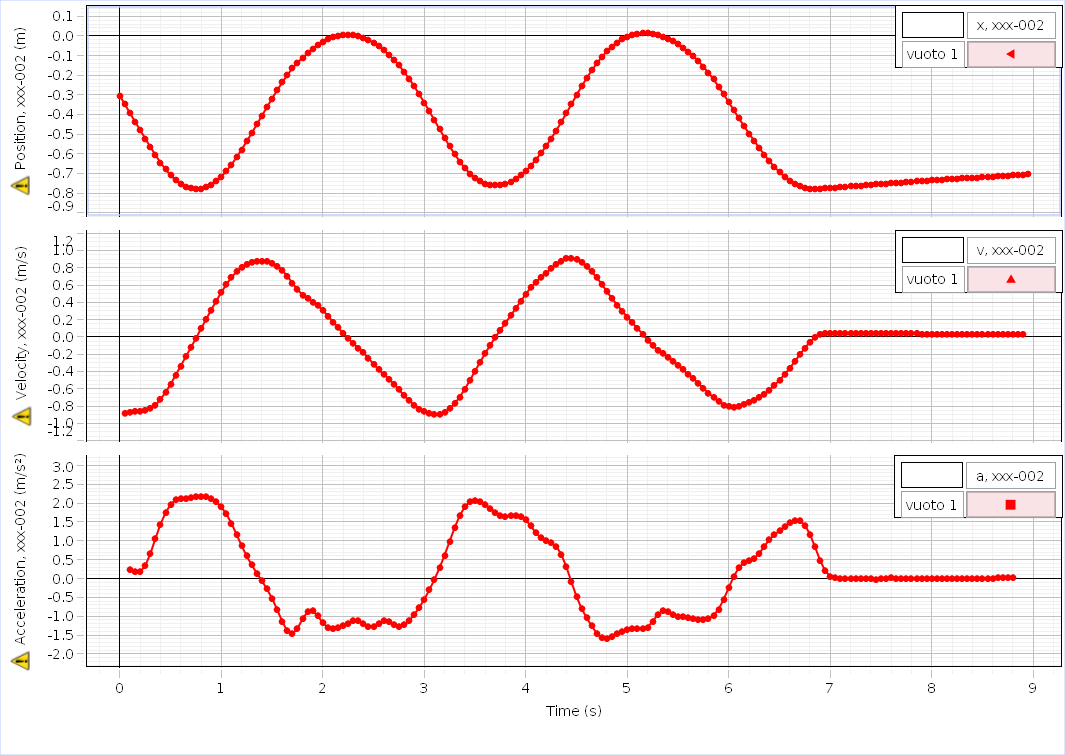
\includegraphics[scale=0.45]{capstone_data/vuoto_1.png}
				\end{subfigure}%
				
				\begin{subfigure}{0.9\textwidth}
					\caption{carrello rosso caricato con 500g}
					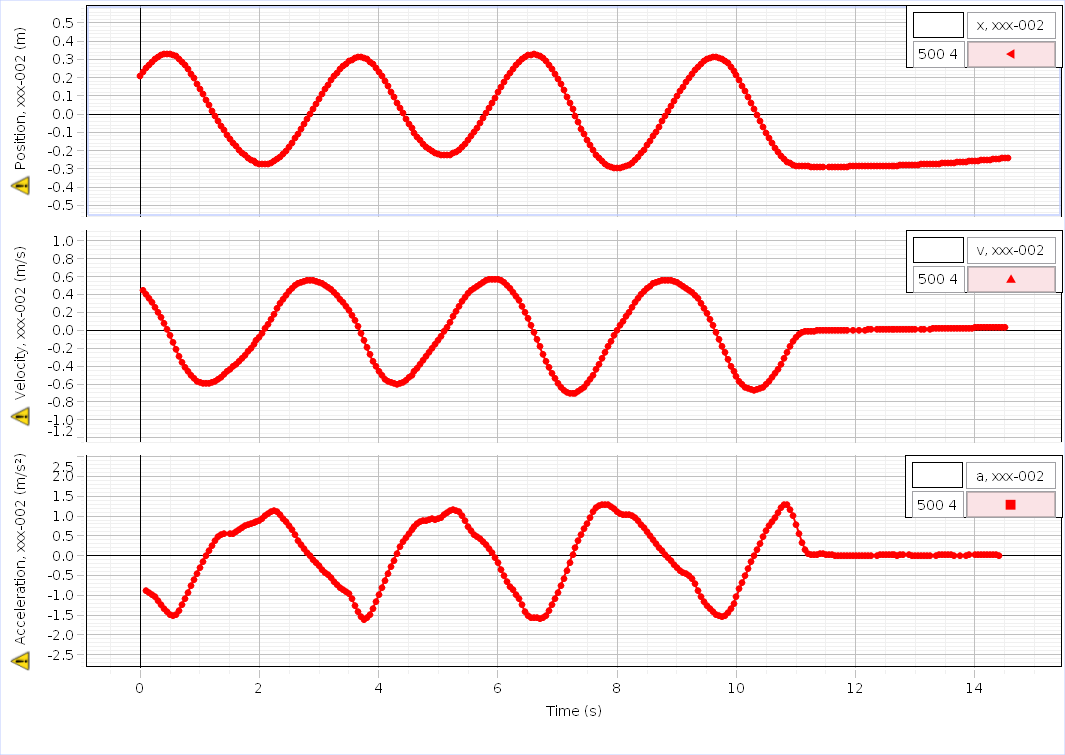
\includegraphics[scale=0.45]{capstone_data/500_4.png}
				\end{subfigure}%
			}
		}
\end{figure}
	
	\begin{figure}[!htbp]
		\captionsetup{labelformat=empty}
		\caption{Grafici velocità e accelerazione in funzione della posizione}
		\makebox[1 \textwidth][c]{       %centering table
			\resizebox{1.40 \textwidth}{!}{
				\begin{subfigure}{0.9\textwidth}
					\caption{carrello rosso vuoto}
					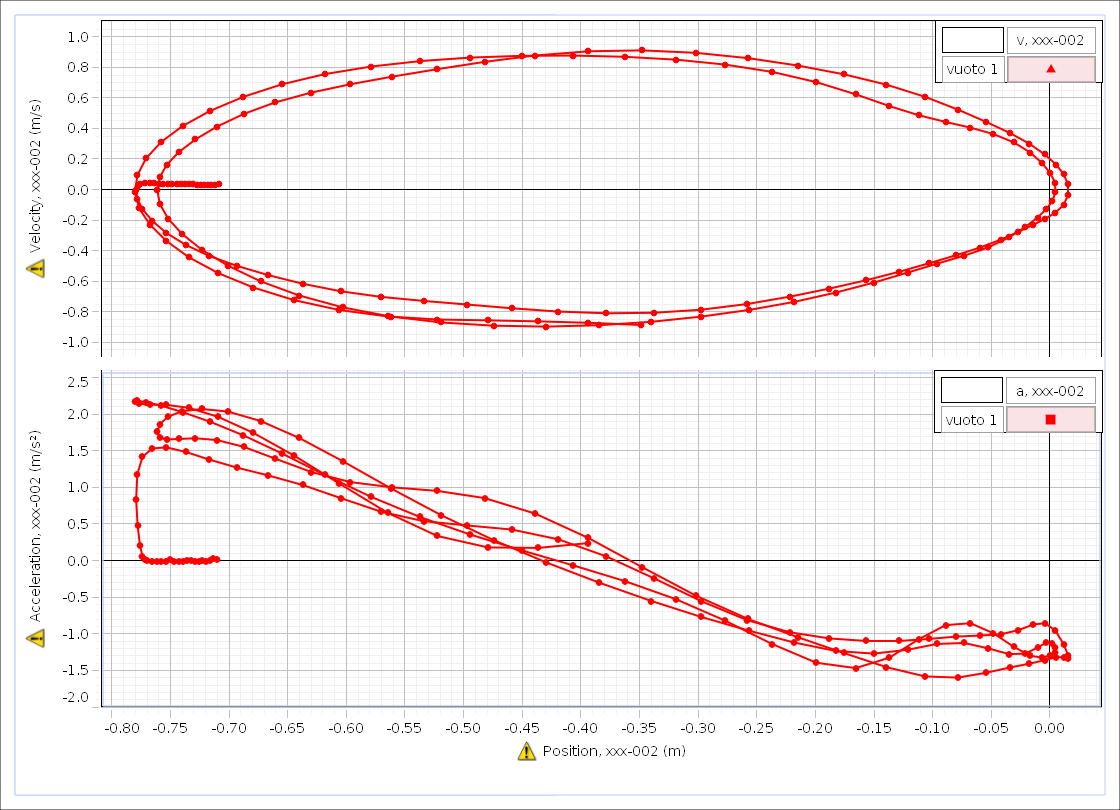
\includegraphics[scale=0.45]{capstone_data/vuoto_1_vel_acc.png}
				\end{subfigure}%
				
				\begin{subfigure}{0.9\textwidth}
					\caption{carrello rosso caricato con 500g}
					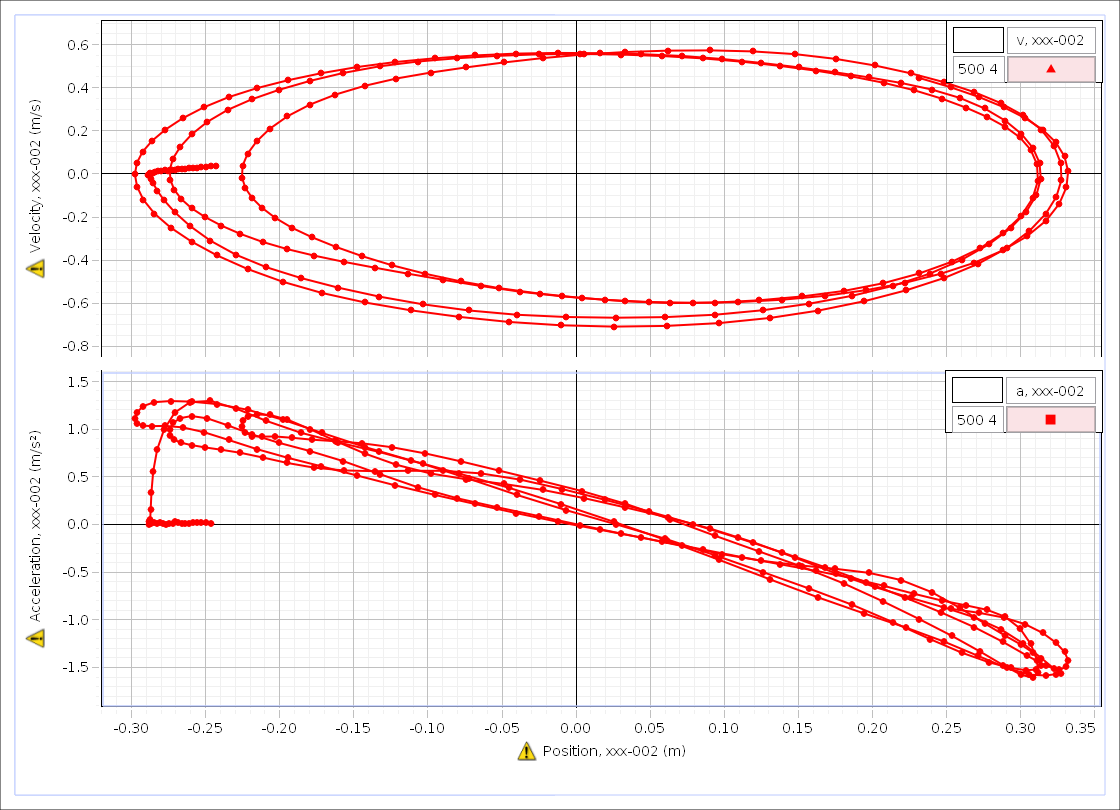
\includegraphics[scale=0.45]{capstone_data/500_4_vel_acc.png}
				\end{subfigure}%
			}
		}
	\end{figure}

\subsection*{verifica della legge di Newton}


\begin{figure}[!htbp]
	\captionsetup{labelformat=empty}
	\caption{massa del carrello rosso in grammi}
	\makebox[1 \textwidth][c]{       %centering table
		\begin{tabular}{cccccccc}
			\hline
			\hline
			252.64 &252.63 & 252.62 &252.63& 252.62 & 252.62 & 252.62 & 252.62\\
			
			\hline
			\hline
		\end{tabular}
	}
	\caption{\(\bar{m} = 252.63 g\)}
\end{figure}

	\begin{figure}[!htbp]
		\captionsetup{labelformat=empty}
		\caption{grafici \(F_{(a)}\) per il carrello rosso vuoto}
		\makebox[1 \textwidth][c]{       %centering table
			\resizebox{1.0 \textwidth}{!}{
				\begin{subfigure}{0.9\textwidth}
					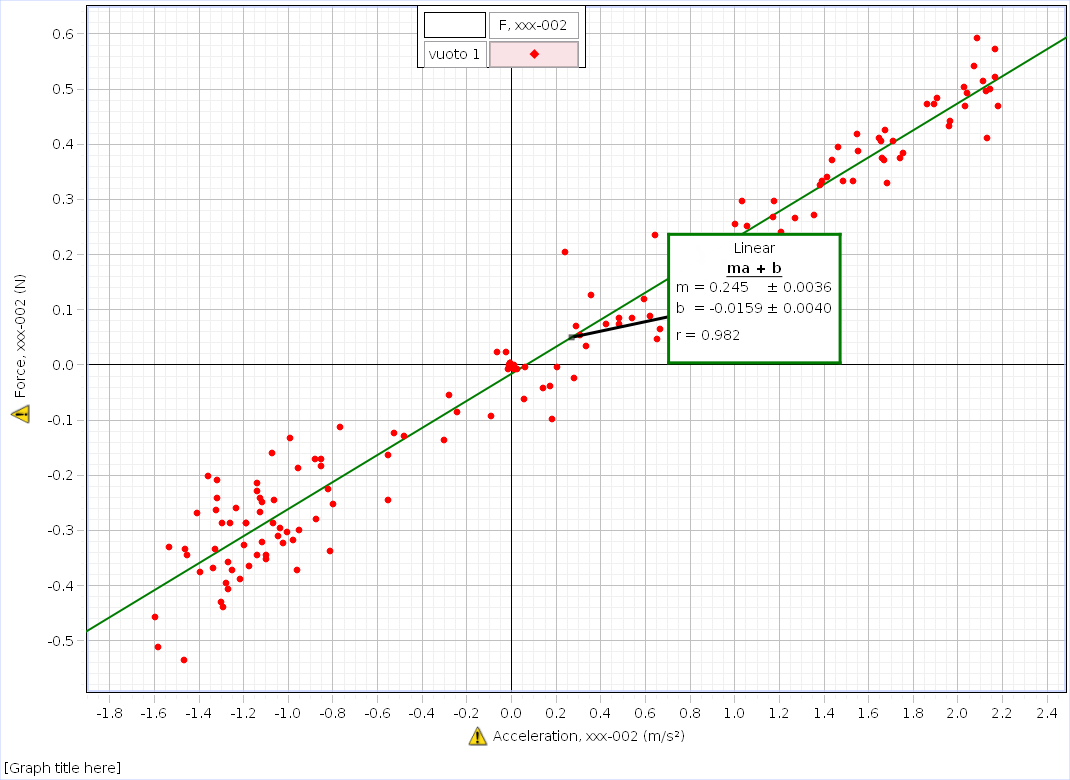
\includegraphics[scale=0.45]{capstone_data/vuoto1.png}
				\end{subfigure}%
				
				\begin{subfigure}{0.9\textwidth}
					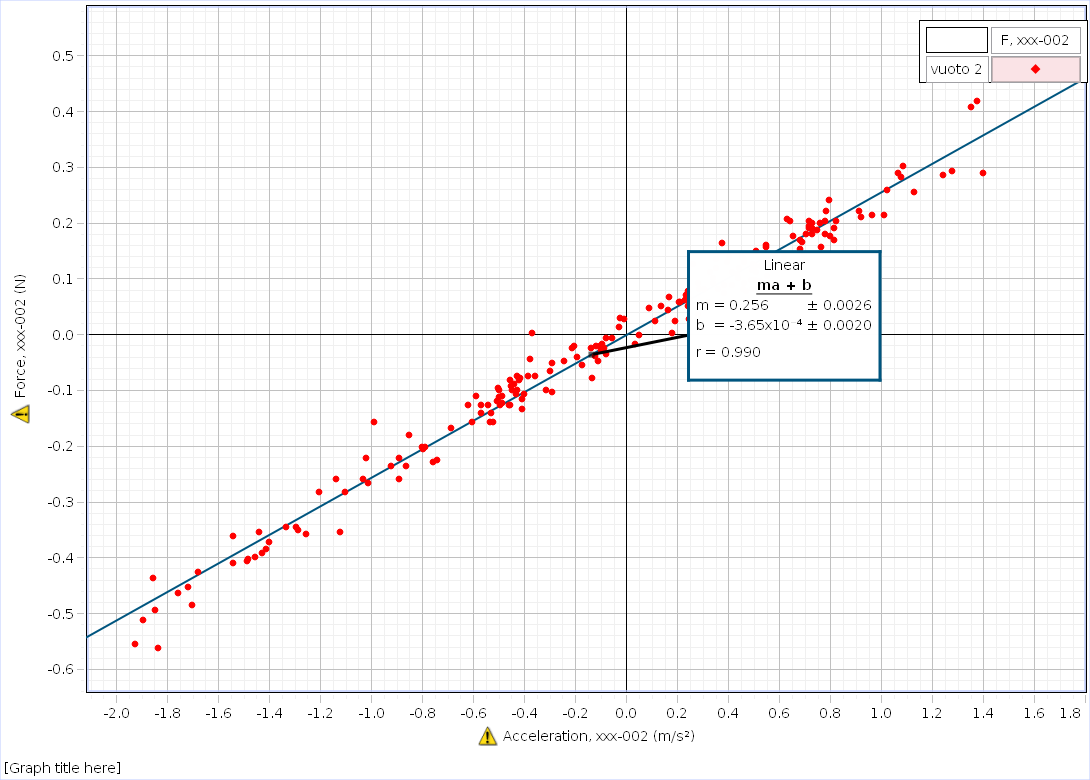
\includegraphics[scale=0.45]{capstone_data/vuoto2.png}
				\end{subfigure}%
			}
		}
	\end{figure}

\begin{figure}[!htbp]
	\makebox[1 \textwidth][c]{       %centering table
		\resizebox{1.40 \textwidth}{!}{
			\begin{subfigure}{0.9\textwidth}
				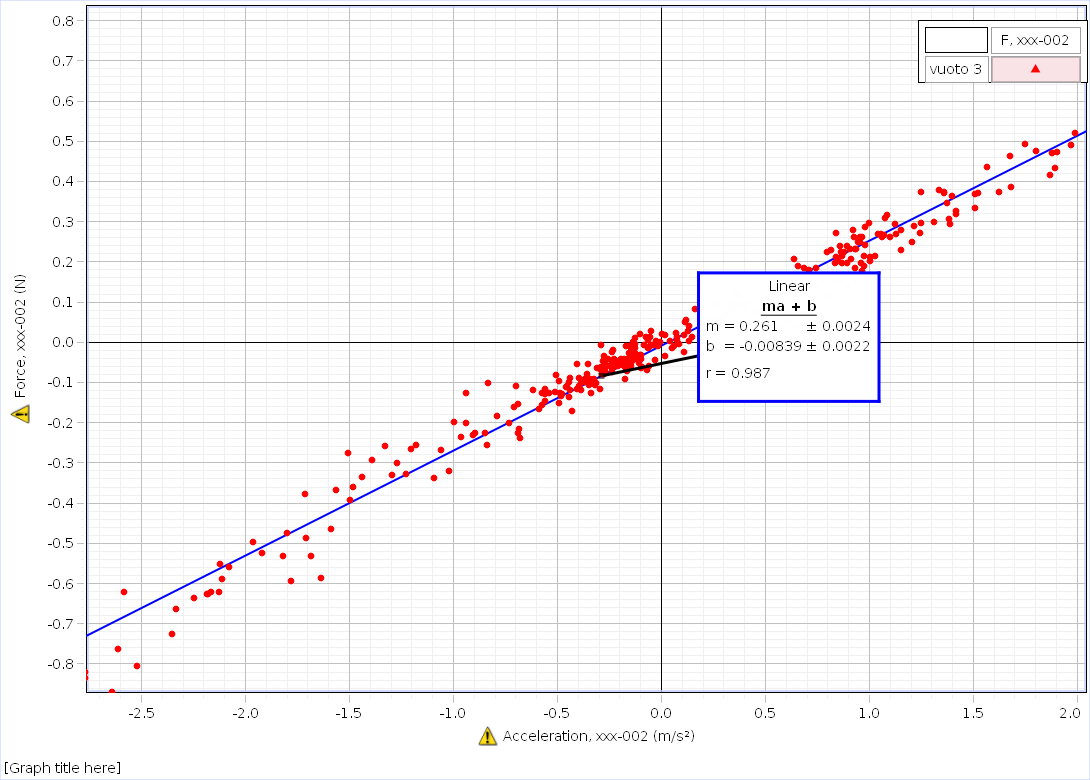
\includegraphics[scale=0.45]{capstone_data/vuoto3.png}
			\end{subfigure}%
			
			\begin{subfigure}{0.9\textwidth}
				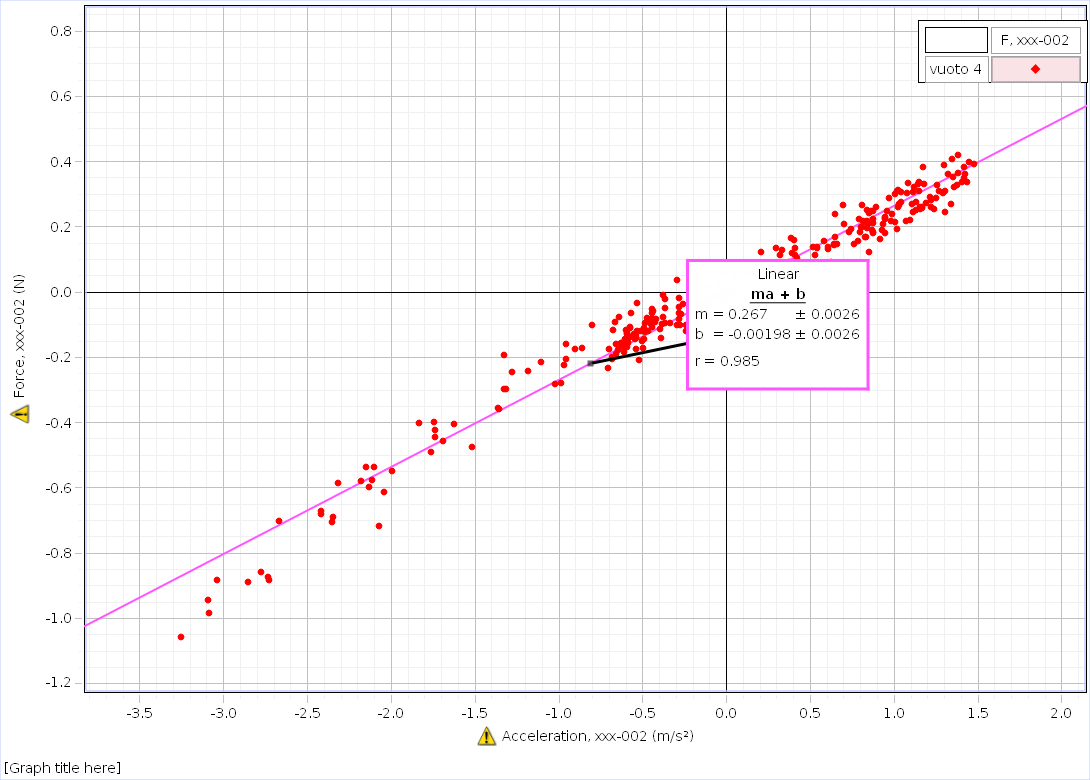
\includegraphics[scale=0.45]{capstone_data/vuoto4.png}
			\end{subfigure}%
			
			\begin{subfigure}{0.9\textwidth}
			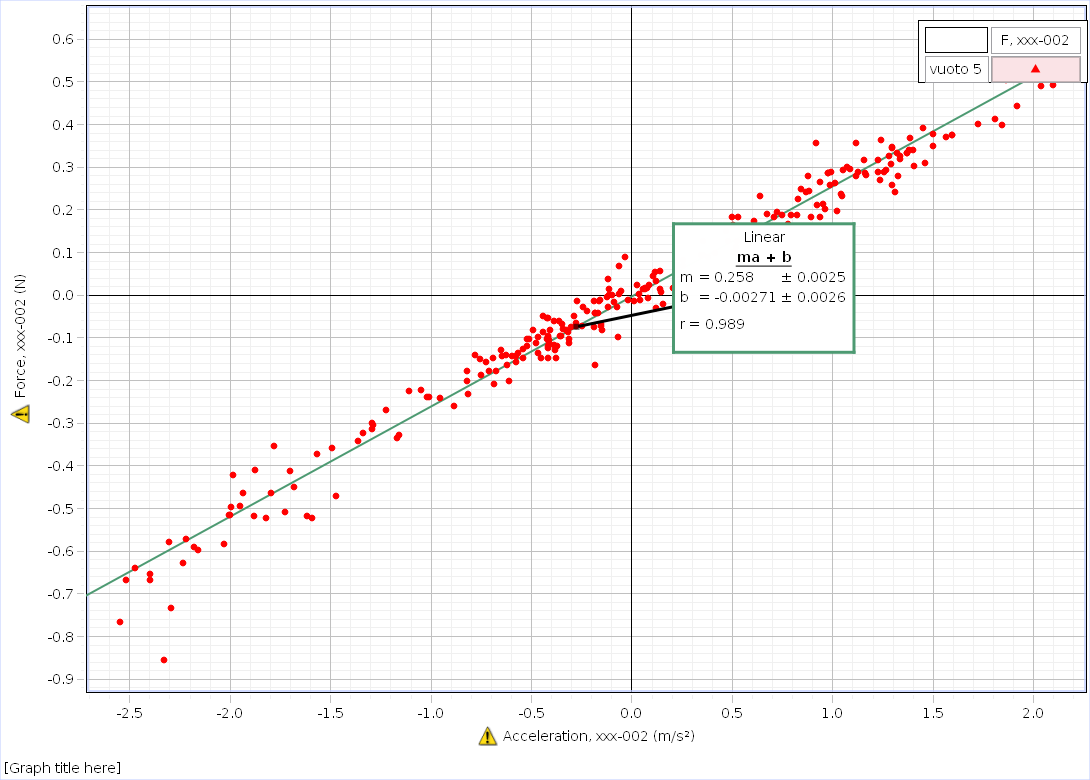
\includegraphics[scale=0.45]{capstone_data/vuoto5.png}
			\end{subfigure}%
		}
	}
\end{figure}


\begin{figure}[!htbp]
	\captionsetup{labelformat=empty}
	\caption{}
	\makebox[1 \textwidth][c]{       %centering table
		\begin{tabular}{c|c}
			run & coefficiente angolare = m (Kg)\\
			\hline
			1: & \(0.245 \pm 0.0036\)\\
			\hline
			2: &\(0.256 \pm 0.0026\)\\
			\hline
			3: &\(0.261 \pm 0.0024\)\\
			\hline
			4: &\(0.267 \pm 0.0026\)\\
			\hline
			5: &\(0.258 \pm 0.0025\)\\
			\hline
		\end{tabular}
	}
	\caption{\(\bar{m} = 0.259 \pm 0.001 Kg\)}
	
\end{figure}
la media delle masse è stata calcolata con \(\bar{m} = \frac{\sum x_{i}w_{i}}{\sum w_{i}} \pm \frac{1}{\sqrt{\sum w_{i}}}\)

\[t = \frac{\left | m_{osservata} - m_{attesa} \right |}{\sigma_{m}}= 6.37\]\\
\noindent \(\rightarrow\) la probabilità che la differenza sia dovuta solo ad errori casuali è inferiore al 0.3 \(\%\).
	
\begin{figure}[!htbp]
	\captionsetup{labelformat=empty}
	\caption{massa del pesetto da 500g grammi}
	\makebox[1 \textwidth][c]{       %centering table
		\begin{tabular}{cccccccc}
			\hline
			\hline
			506.36 &506.37& 506.37&506.38&506.38&506.38&506.38&506.37\\
			\hline
			\hline
		\end{tabular}
	}
	\caption{\(\bar{m} = 506.37 g\)}
	\caption{massa totale carrello rosso+pesetto da 500g = 759g.}
\end{figure}

\begin{figure}[!htbp]
			\captionsetup{labelformat=empty}
	\caption{grafici \(F_{(a)}\) per il carrello rosso caricato di 500g}
	\makebox[1 \textwidth][c]{       %centering table
		\resizebox{1.0 \textwidth}{!}{
			\begin{subfigure}{0.9\textwidth}
				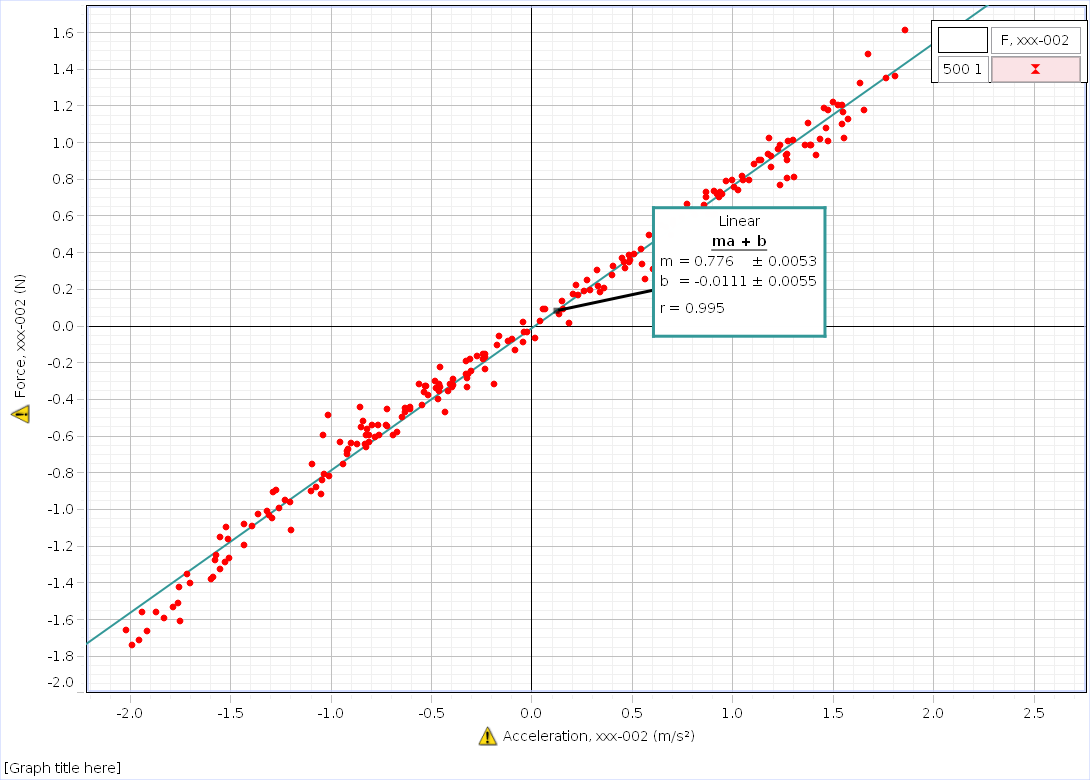
\includegraphics[scale=0.45]{capstone_data/5001.png}
			\end{subfigure}%
			
			\begin{subfigure}{0.9\textwidth}
				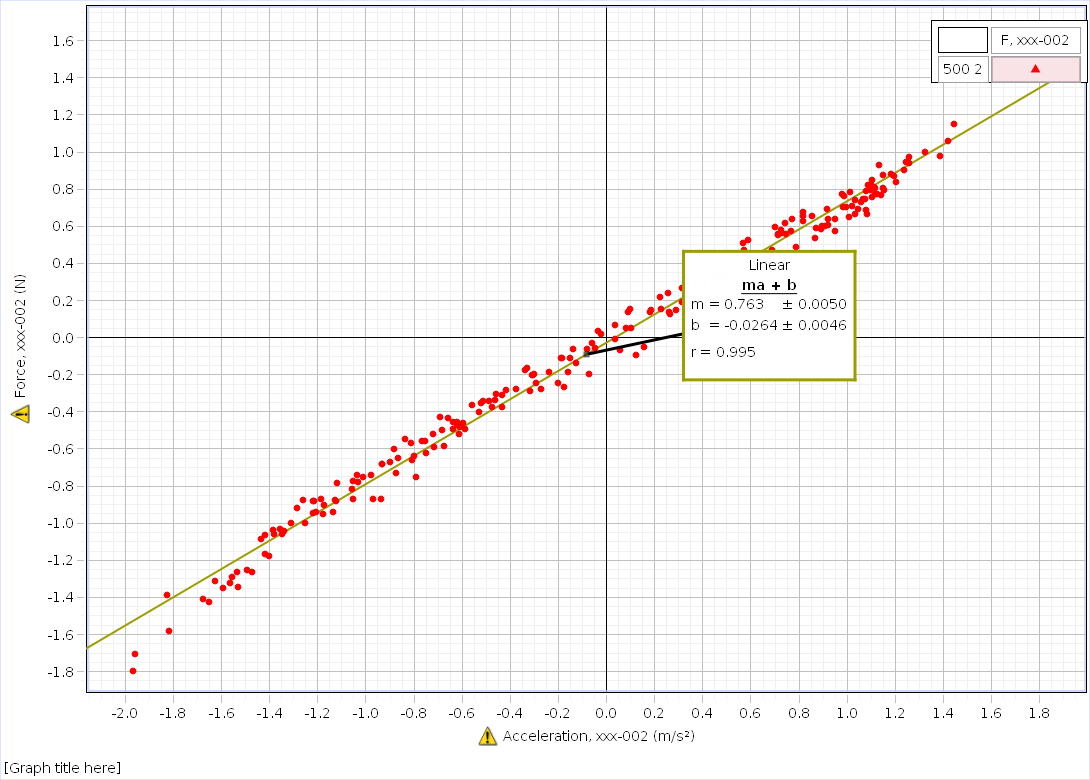
\includegraphics[scale=0.45]{capstone_data/5002.png}
			\end{subfigure}%
		}
	}
\end{figure}

\begin{figure}[!htbp]
	\makebox[1 \textwidth][c]{       %centering table
		\resizebox{1.40 \textwidth}{!}{
			\begin{subfigure}{0.9\textwidth}
				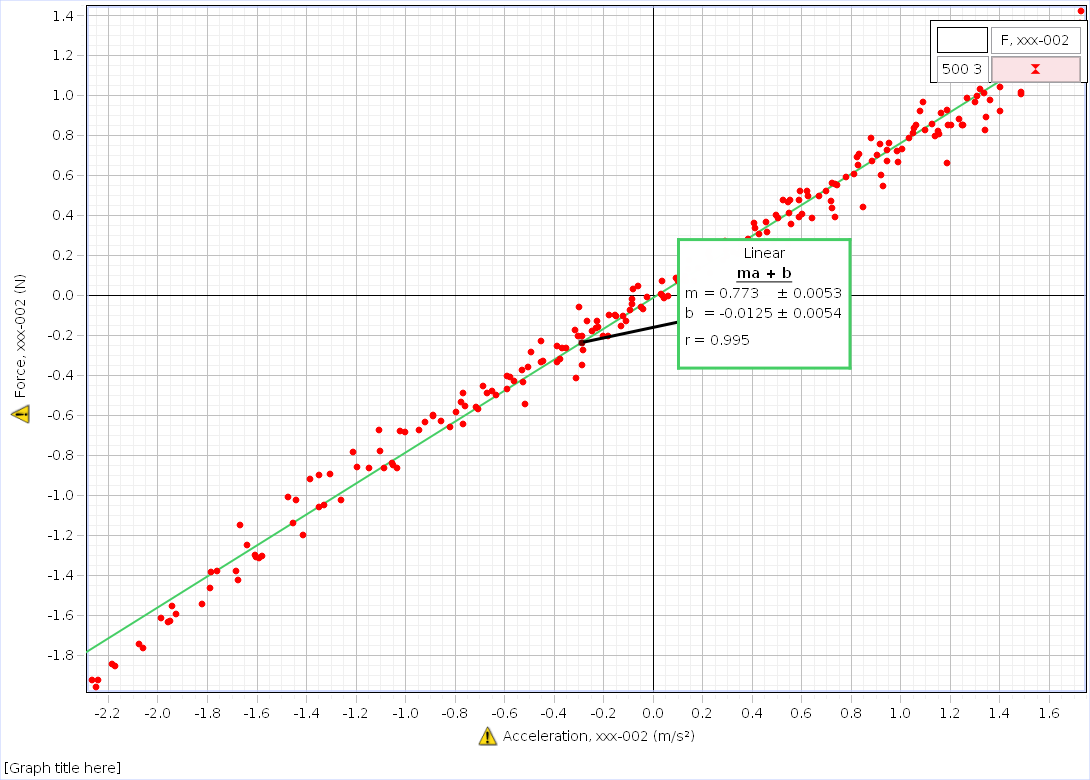
\includegraphics[scale=0.45]{capstone_data/5003.png}
			\end{subfigure}%
			
			\begin{subfigure}{0.9\textwidth}
				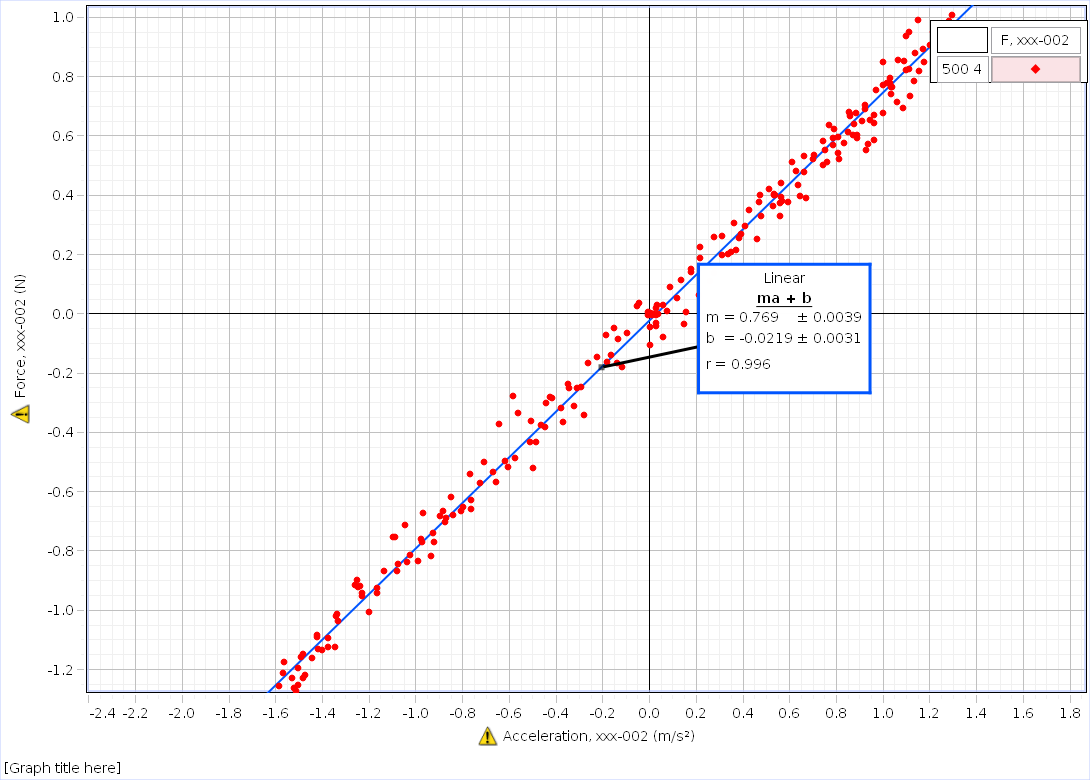
\includegraphics[scale=0.45]{capstone_data/5004.png}
			\end{subfigure}%
			
			\begin{subfigure}{0.9\textwidth}
				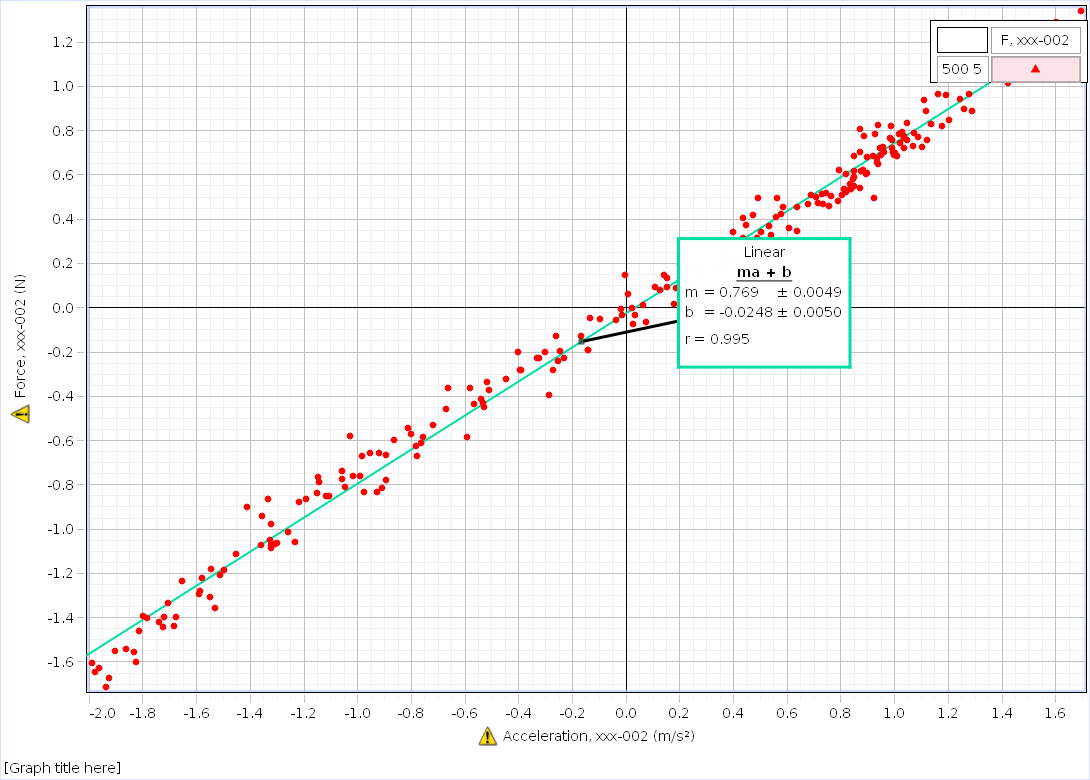
\includegraphics[scale=0.45]{capstone_data/5005.png}
			\end{subfigure}%
		}
	}
\end{figure}

\begin{figure}[!htbp]
	\captionsetup{labelformat=empty}

	\makebox[1 \textwidth][c]{       %centering table
		\begin{tabular}{c|c}
			run & coefficiente angolare=m (Kg)\\
			\hline
			1:& \(0.776 \pm 0.005\)\\
			\hline
			2:&\(0.763 \pm 0.005\)\\
			\hline
			3:& \(0.773 \pm 0.005\)\\
			\hline
			4:& \(0.769 \pm 0.004\)\\
			\hline
			5:& \(0.769 \pm 0.005\)\\
		\end{tabular}
	}
	\caption{\(\bar{m} =  0.770 \pm 0.002 Kg\)}
	
\end{figure}

\[t = \frac{\left | m_{osservata} - m_{attesa} \right |}{\sigma_{m}}= 5.5\]\\
\noindent \(\rightarrow\) la probabilità che la differenza sia dovuta solo ad errori casuali è inferiore al 0.3 \(\%\).

	\begin{figure}[!htbp]
	\captionsetup{labelformat=empty}
	\caption{grafici \(F_{(a)}\) per il carrello rosso su piano inclinato di \(\theta = 5^{\circ}\)}
	\makebox[1 \textwidth][c]{       %centering table
		\resizebox{1.0 \textwidth}{!}{
			\begin{subfigure}{0.9\textwidth}
				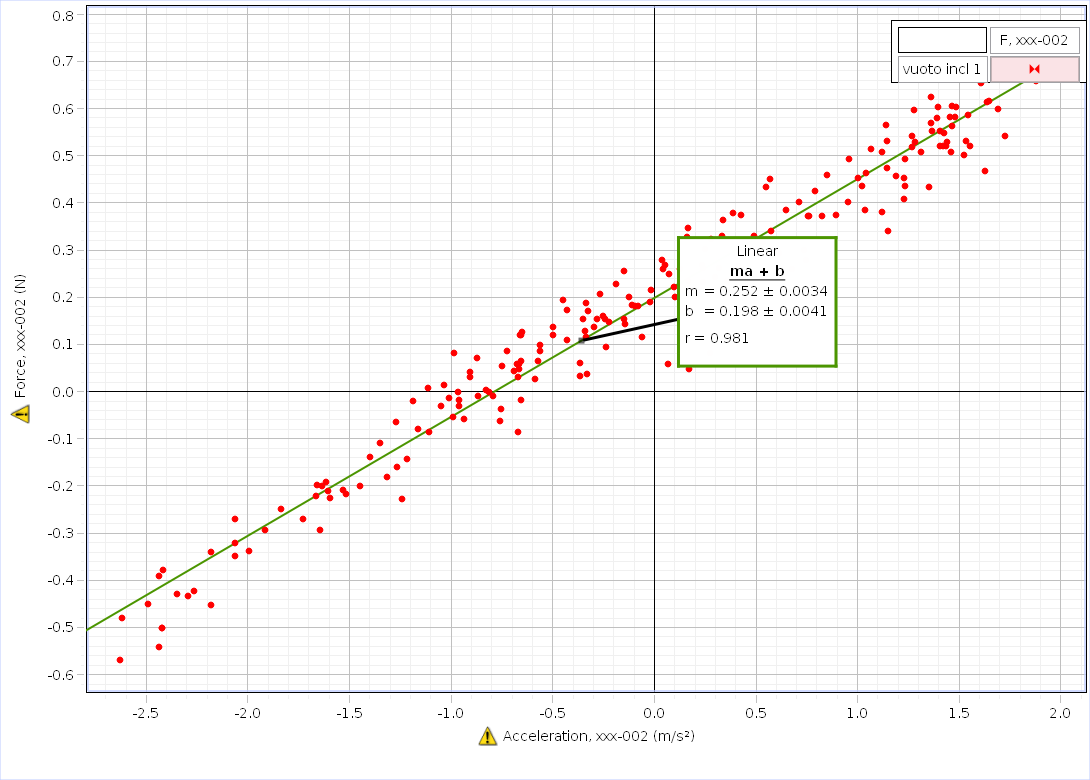
\includegraphics[scale=0.45]{capstone_data/incl1.png}
			\end{subfigure}%
			
			\begin{subfigure}{0.9\textwidth}
				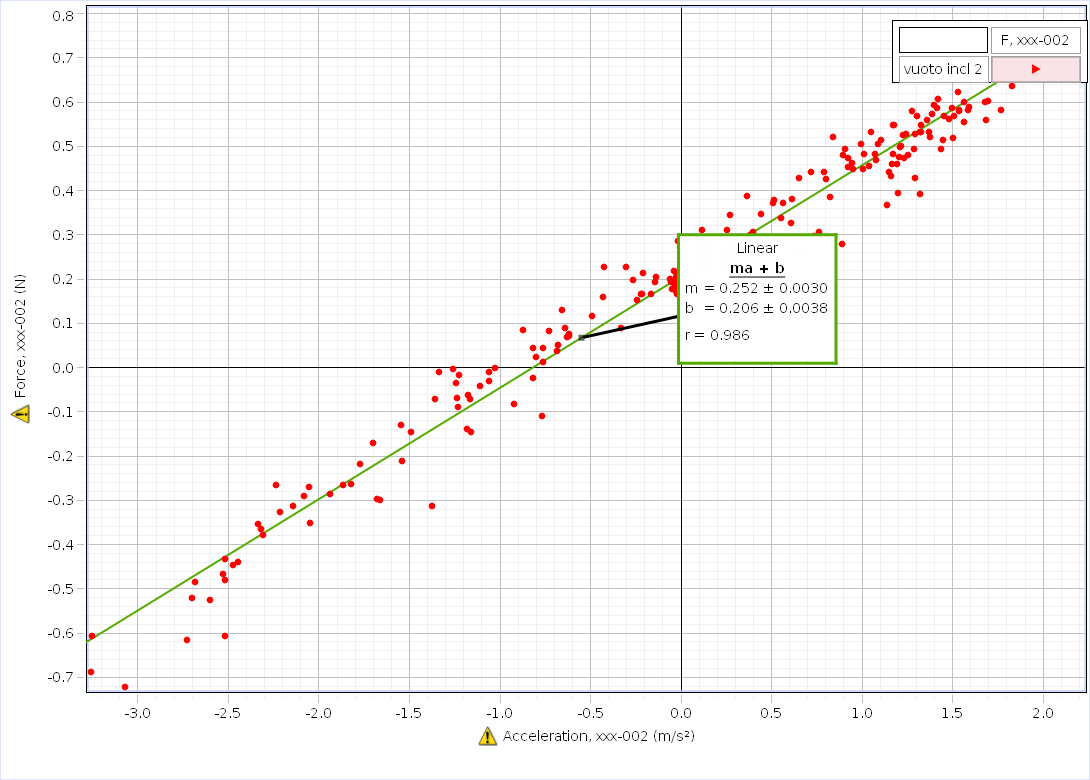
\includegraphics[scale=0.45]{capstone_data/incl2.png}
			\end{subfigure}%
		}
	}
\end{figure}

\begin{figure}[!htbp]
		\captionsetup{labelformat=empty}
	\makebox[1 \textwidth][c]{       %centering table
		\resizebox{1.40 \textwidth}{!}{
			\begin{subfigure}{0.9\textwidth}
				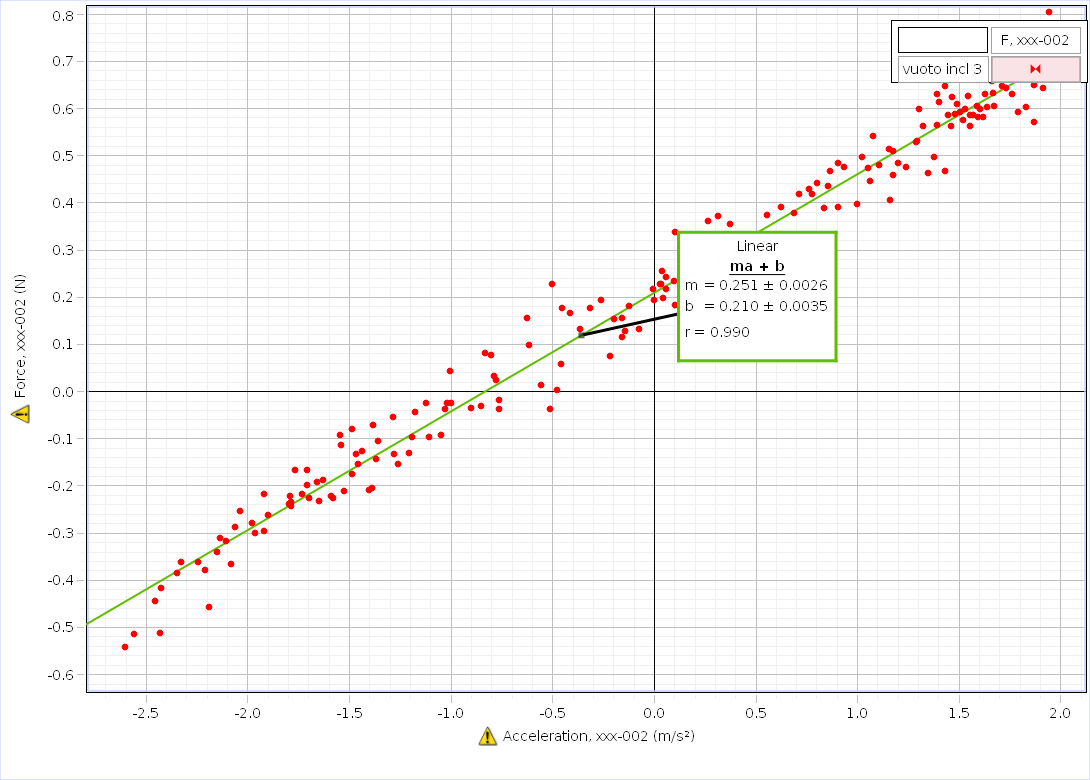
\includegraphics[scale=0.45]{capstone_data/incl3.png}
			\end{subfigure}%
			
			\begin{subfigure}{0.9\textwidth}
				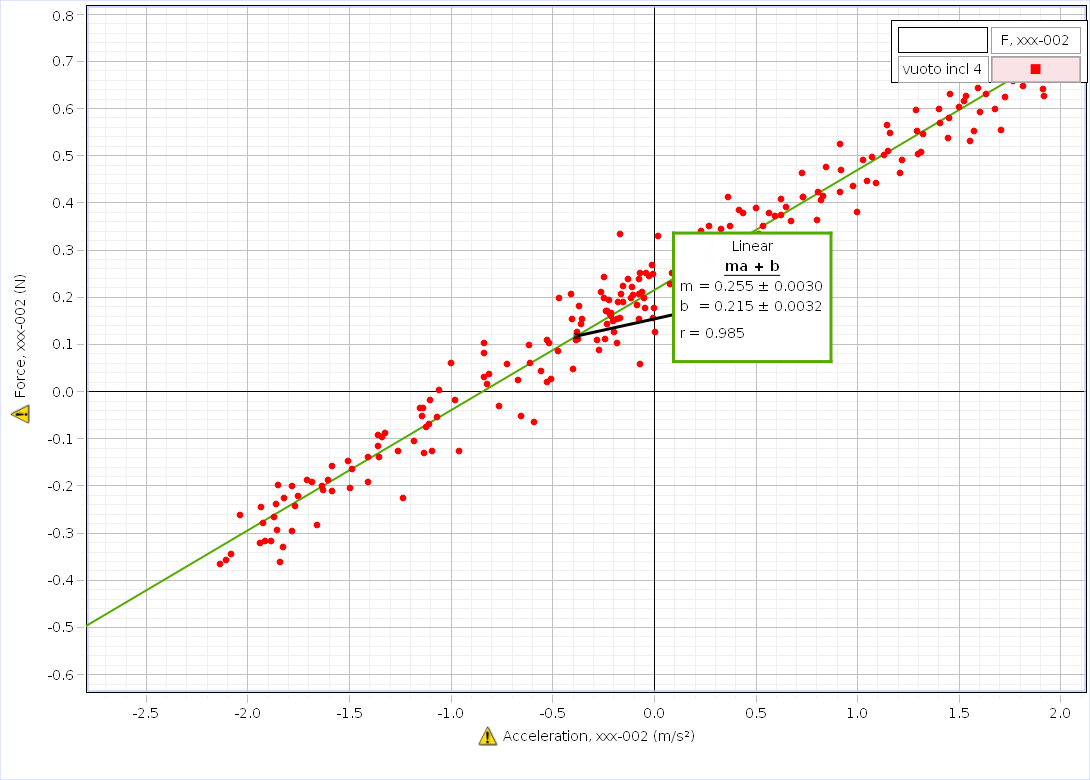
\includegraphics[scale=0.45]{capstone_data/incl4.png}
			\end{subfigure}%
			
			\begin{subfigure}{0.9\textwidth}
				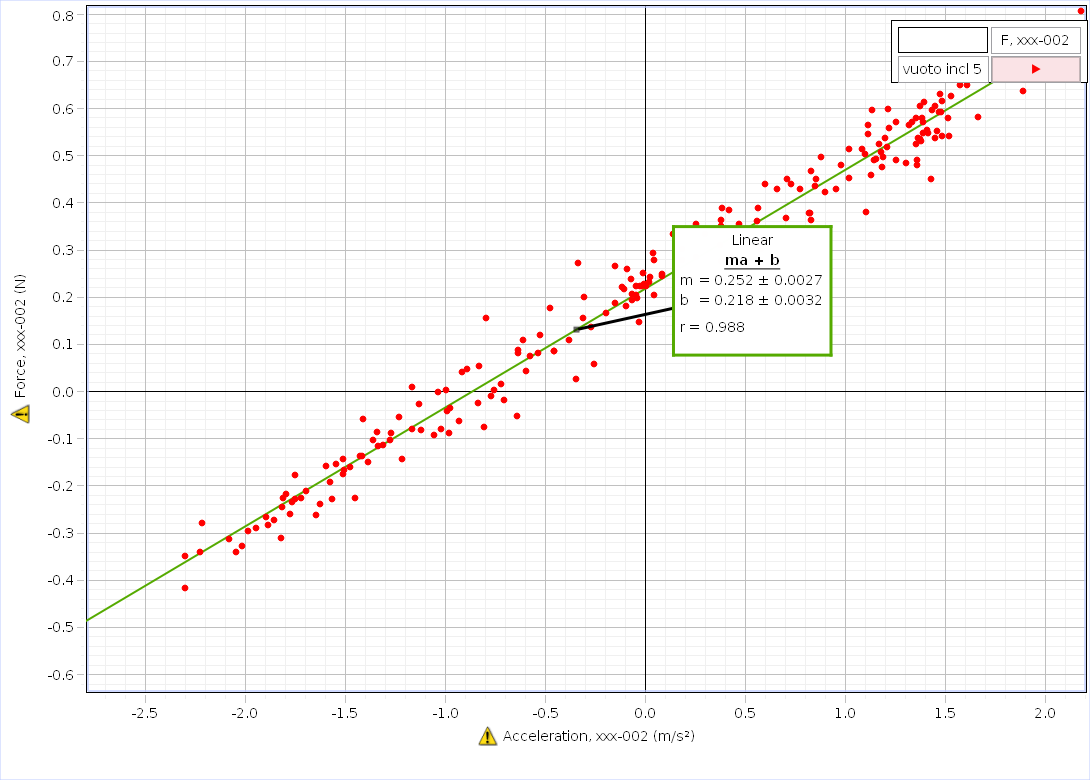
\includegraphics[scale=0.45]{capstone_data/incl5.png}
			\end{subfigure}%
		}
	}
\end{figure}
\begin{figure}[!htbp]
		\captionsetup{labelformat=empty}
	\makebox[1 \textwidth][c]{       %centering table
		\begin{tabular}{c|c|c}
			run & coefficiente angolare=m (Kg) & intercetta = -mgsin(\(\theta\)) (Kg m/\(s^2\))\\
			\hline
			1:& \(0.252 \pm 0.003\) & \(0.198 \pm 0.004\)\\
			\hline
			2:&\(0.252 \pm 0.003\) & \(0.206 \pm 0.004\)\\
			\hline
			3:& \(0.251 \pm 0.003\) & \(0.210 \pm 0.004\)\\
			\hline
			4:& \(0.255 \pm 0.003\) & \(0.215 \pm 0.003\)\\
			\hline
			5:& \(0.252 \pm 0.003\) & \(0.218 \pm 0.003\)\\
			\hline
		\end{tabular}
	}
	\caption{\(\bar{m} = 0.252 \pm 0.001\quad \bar{\theta} =  -4.89 \pm 0.03^{\circ}\)}
\caption{\( con \quad \sigma_{\theta} = arcsin(\frac{\sigma_{A}}{gm})\)}
\end{figure}
\[t = \frac{\left | m_{osservata} - m_{attesa} \right |}{\sigma_{m}}= 0.63\]\\

\noindent \(\rightarrow\) la probabilità che la differenza sia dovuta solo ad errori casuali è del 52.9\(\%\).\\\\
\[t = \frac{\left | \theta_{osservato} - \theta_{atteso} \right |}{\sigma_{\theta}}= 3.7\]\\
\noindent \(\rightarrow\) la probabilità che la differenza sia dovuta solo ad errori casuali è inferiore al 0.3 \(\%\).


\subsection*{urti centrali}

\begin{figure}[!htbp]
\captionsetup{labelformat= empty}
\captionsetup[sub]{font=huge}

		\caption{Grafici molla run 1 in funzione del tempo}
	\makebox[1 \textwidth][c]{       %centering table
		\resizebox{1.60 \textwidth}{!}{
			\begin{subfigure}{1.4\textwidth}
				\caption{posizione}
				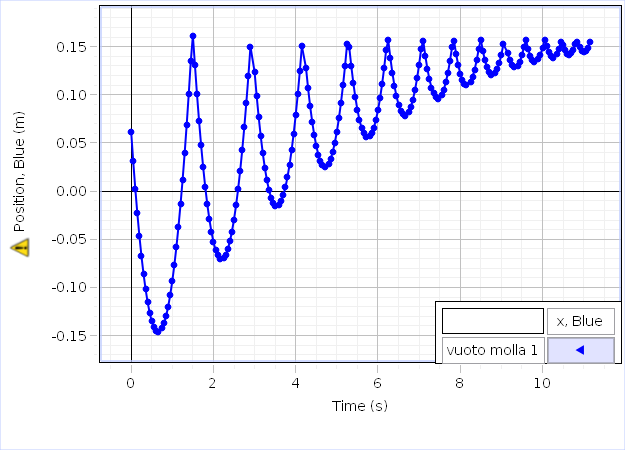
\includegraphics[scale=1.2]{capstone_data/molla_1_pos.png}
			\end{subfigure}%
			
			\begin{subfigure}{1.4\textwidth}
				\caption{velocità}
				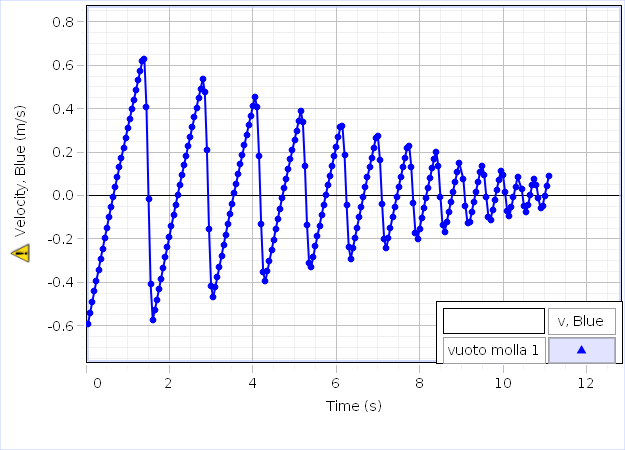
\includegraphics[scale=1.2]{capstone_data/molla_1_vel.png}
			\end{subfigure}%
			
			\begin{subfigure}{1.4\textwidth}
				\caption{accelerazione}
				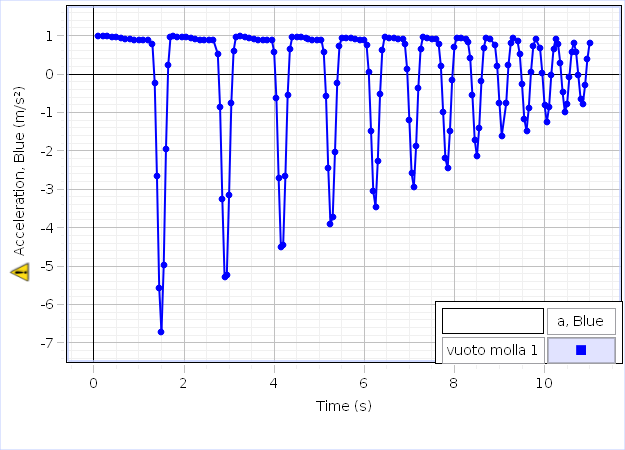
\includegraphics[scale=1.2]{capstone_data/molla_1_acc.png}
			\end{subfigure}%
		}
	}
\end{figure}


\begin{figure}[!htbp]
	\captionsetup{labelformat= empty}
	\captionsetup[sub]{font=huge}
	
	\caption{Grafici magnete run 1 in funzione del tempo}
	\makebox[1 \textwidth][c]{       %centering table
		\resizebox{1.60 \textwidth}{!}{
			\begin{subfigure}{1.4\textwidth}
				\caption{posizione}
				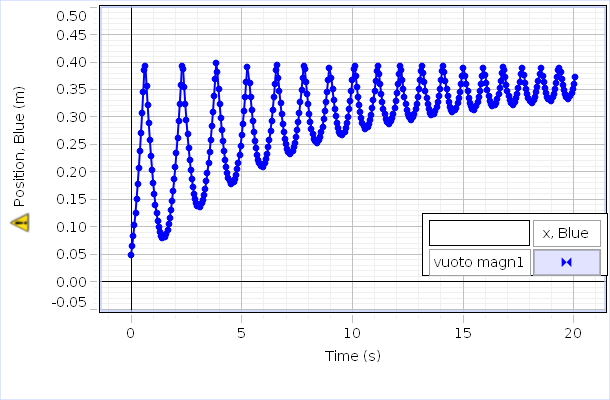
\includegraphics[scale=1.2]{capstone_data/magn_1_pos.png}
			\end{subfigure}%
			
			\begin{subfigure}{1.4\textwidth}
				\caption{velocità}
				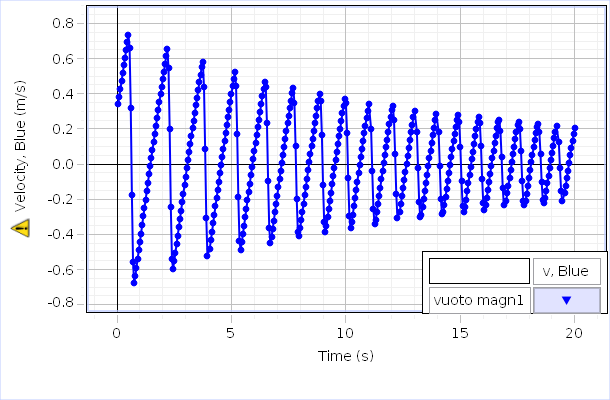
\includegraphics[scale=1.2]{capstone_data/magn_1_vel.png}
			\end{subfigure}%
			
			\begin{subfigure}{1.4\textwidth}
				\caption{accelerazione}
				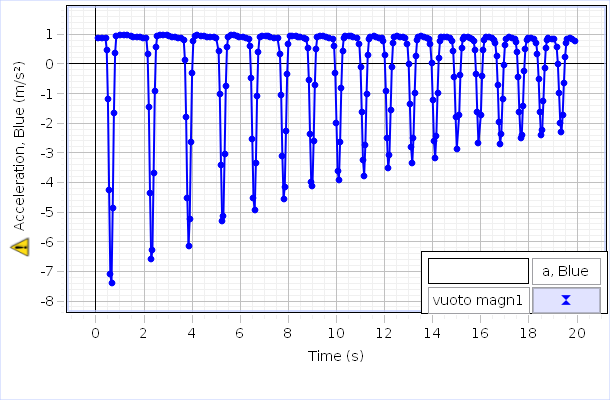
\includegraphics[scale=1.2]{capstone_data/magn_1_acc.png}
			\end{subfigure}%
		}
	}
\end{figure}
.\\\\\\\\\\\\\\\\\\\\\\\\\\
\subsubsection*{verifica del teorema dell'impulso}


\begin{figure}[!htbp]
	\captionsetup{labelformat= empty}
	\captionsetup[sub]{font=LARGE}
	
	\caption{Grafici della quantità di moto, forza e impulso con la molla}
	\makebox[1 \textwidth][c]{       %centering table
		\resizebox{1.70 \textwidth}{!}{
			\begin{subfigure}{2.0\textwidth}
				\caption{run 1}
				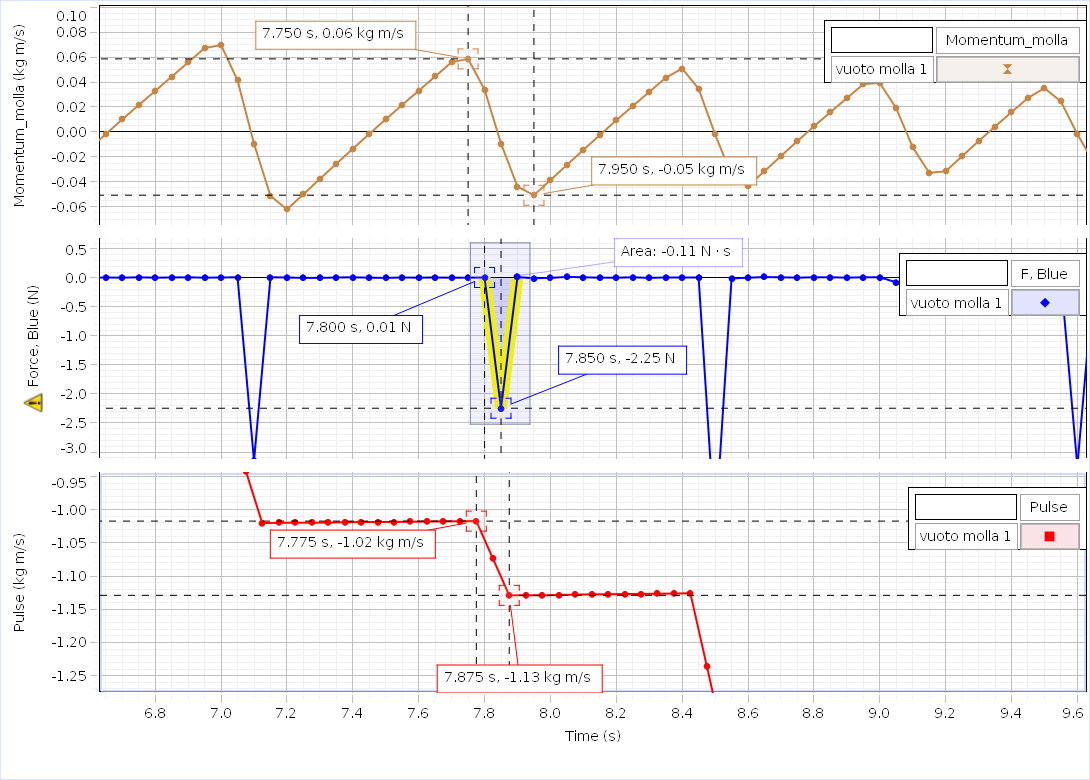
\includegraphics[scale=1.0]{capstone_data/molla_1.png}
			\end{subfigure}%
			
			\begin{subfigure}{2.0\textwidth}
				\caption{run 2}
				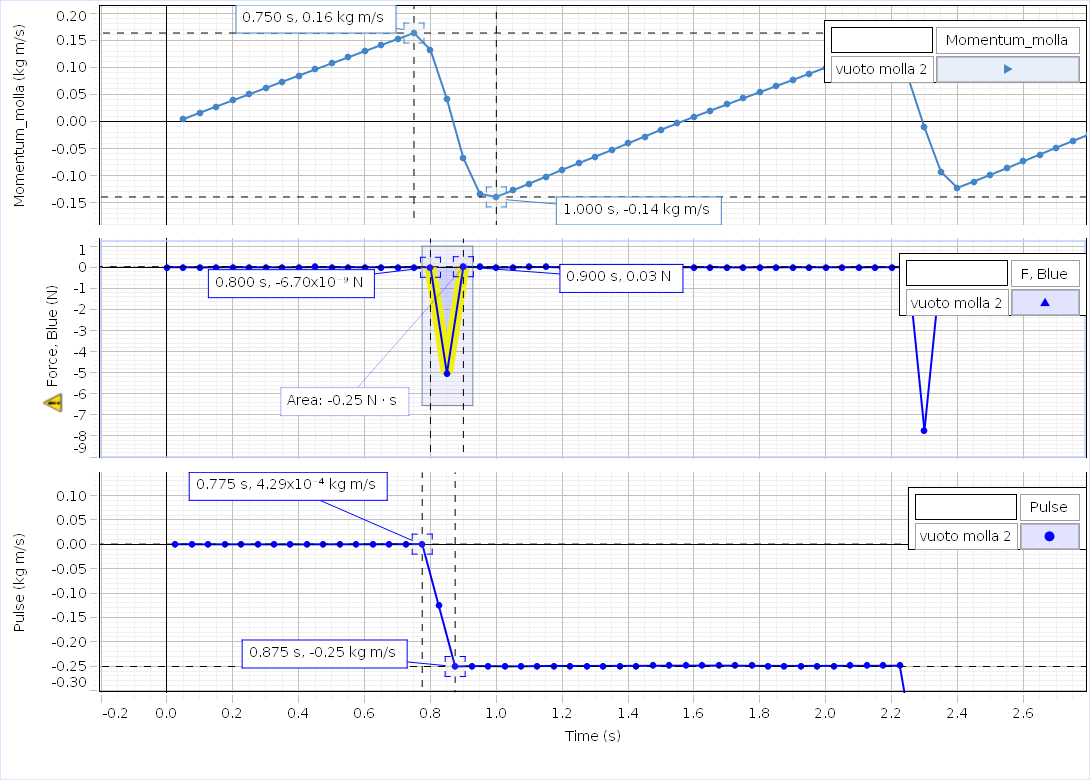
\includegraphics[scale=1.0]{capstone_data/molla_2.png}
			\end{subfigure}%
		}
	}
\end{figure}

\begin{figure}[!htbp]
	\captionsetup{labelformat= empty}
	\captionsetup[sub]{font=huge}
	
	\makebox[1 \textwidth][c]{       %centering table
		\resizebox{1.60 \textwidth}{!}{
			\begin{subfigure}{2.0\textwidth}
				\caption{run3}
				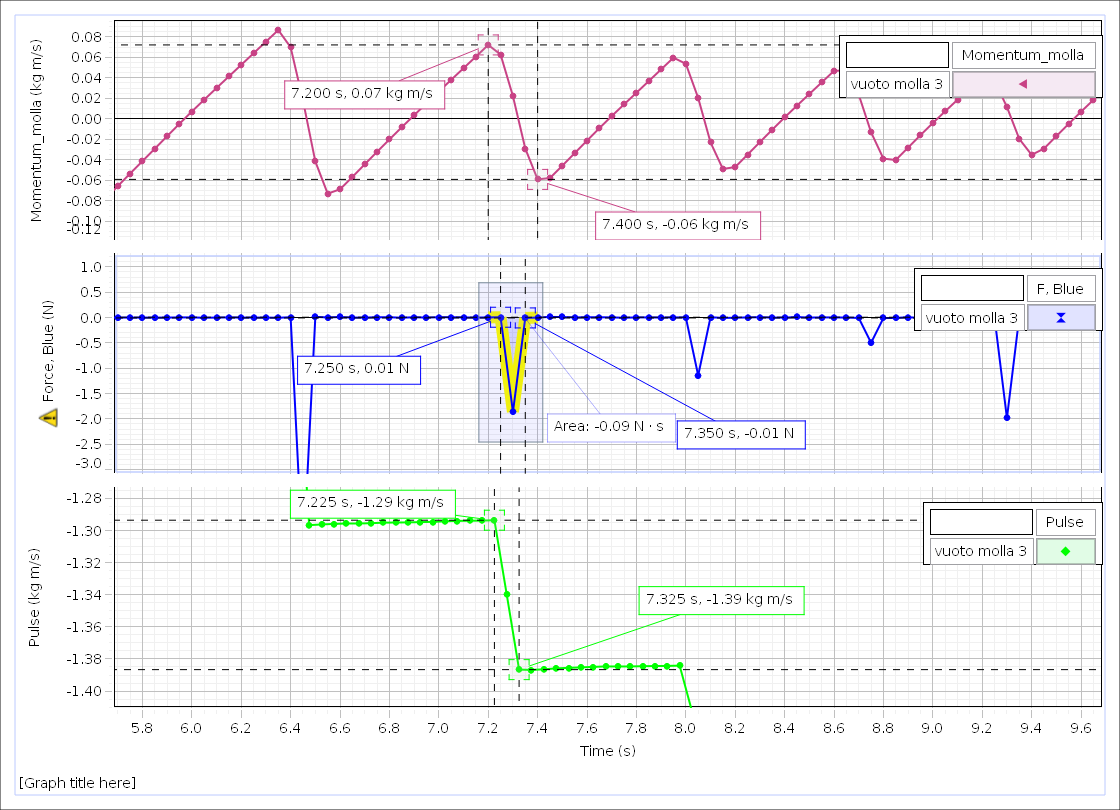
\includegraphics[scale=1.0]{capstone_data/molla_3.png}
			\end{subfigure}%
			
			\begin{subfigure}{2.0\textwidth}
				\caption{run 4}
				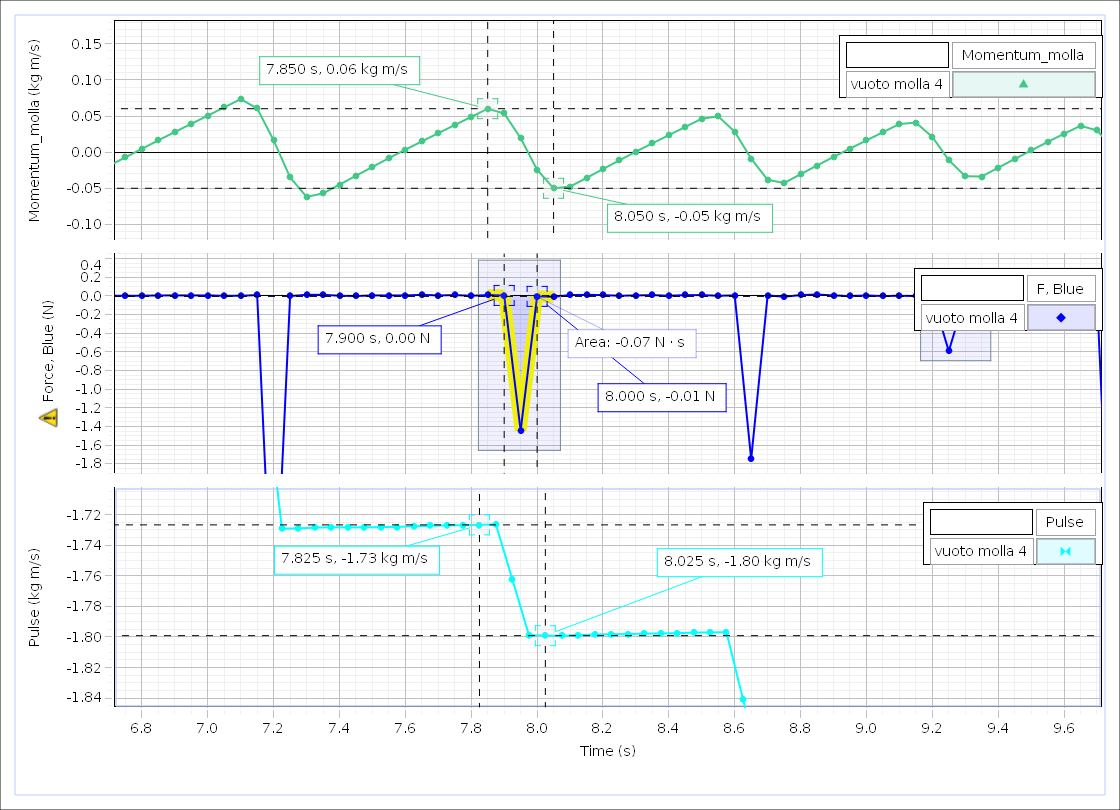
\includegraphics[scale=1.0]{capstone_data/molla_4.png}
			\end{subfigure}%
			
		}
	}
\end{figure}
.\\\\\\\\\\
\begin{figure}[!htbp]
	\captionsetup{labelformat= empty}
	\captionsetup[sub]{font=LARGE}

	\makebox[1 \textwidth][c]{       %centering table
		\resizebox{0.89\textwidth}{!}{
			\begin{subfigure}{2.0\textwidth}
				\caption{run 5}
				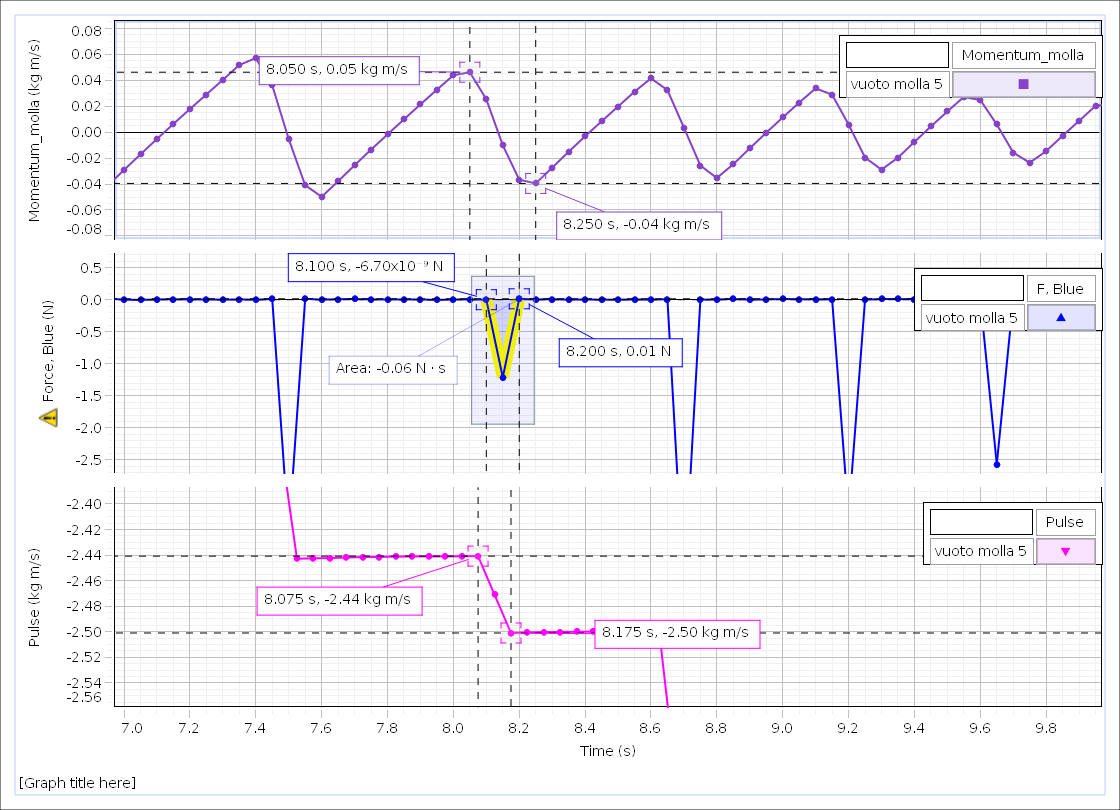
\includegraphics[scale=1.0]{capstone_data/molla_5.png}
			\end{subfigure}%
		}
	}
\end{figure}


\begin{figure}[!htbp]
			\captionsetup{labelformat= empty}
	\caption{verifica teorema dell'impulso con la molla}
	\makebox[1 \textwidth][c]{       %centering table
		\begin{tabular}{||ccc||}
			\hline
			\hline
			run & \(\Delta p\) (Kg m/s) & I (N s)\\
			\hline
			1: & -0.05-0.06 = -0.11 & -0.11\\
			2: & -0.14-0.16 = -0.30 & -0.25\\
			3: & -0.06-0.07 = -0.13 & -0.09\\
			4: & -0.05-0.06 = -0.11 & -0.07\\
			5: & -0.04-0.05 = -0.09 & -0.06\\
			\hline
			\hline
		\end{tabular}
		
	} %close centering
\end{figure}
%----------------------???--------------------
\[t = \frac{\left |\bar{I} - \bar{\Delta p} \right |}{\sqrt{\sigma_{I}^{2}+\sigma_{\Delta p}^{2}}}= \frac{0.032}{\sqrt{0.038^{2}+0.034^{2}}}=0.63\]\\
\noindent \(\rightarrow\) la probabilità che la differenza sia dovuta solo ad errori casuali è del 53\(\%\).\\\\
\begin{figure}[!htbp]
	\captionsetup{labelformat= empty}
	\captionsetup[sub]{font=LARGE}
	
	\caption{Grafici della quantità di moto, forza e impulso con il magnete}
	\makebox[1 \textwidth][c]{       %centering table
		\resizebox{1.70 \textwidth}{!}{
			\begin{subfigure}{2.0\textwidth}
				\caption{run 1}
				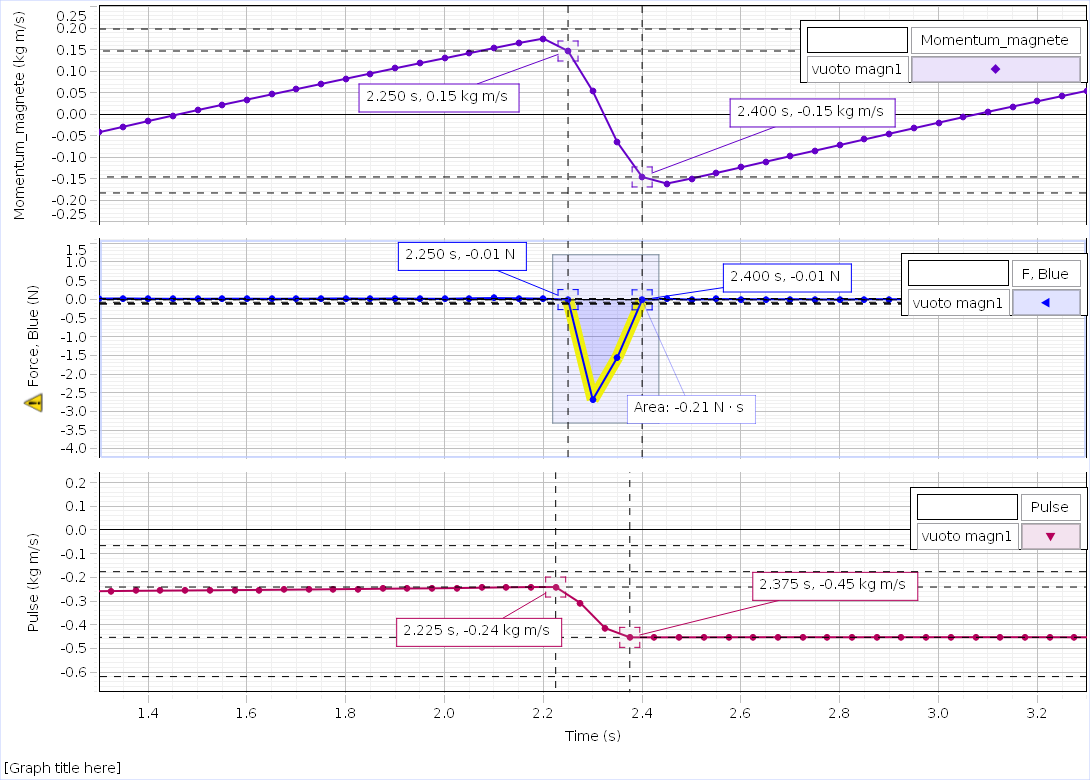
\includegraphics[scale=1.0]{capstone_data/magn_1.png}
			\end{subfigure}%
			
			\begin{subfigure}{2.0\textwidth}
				\caption{run 2}
				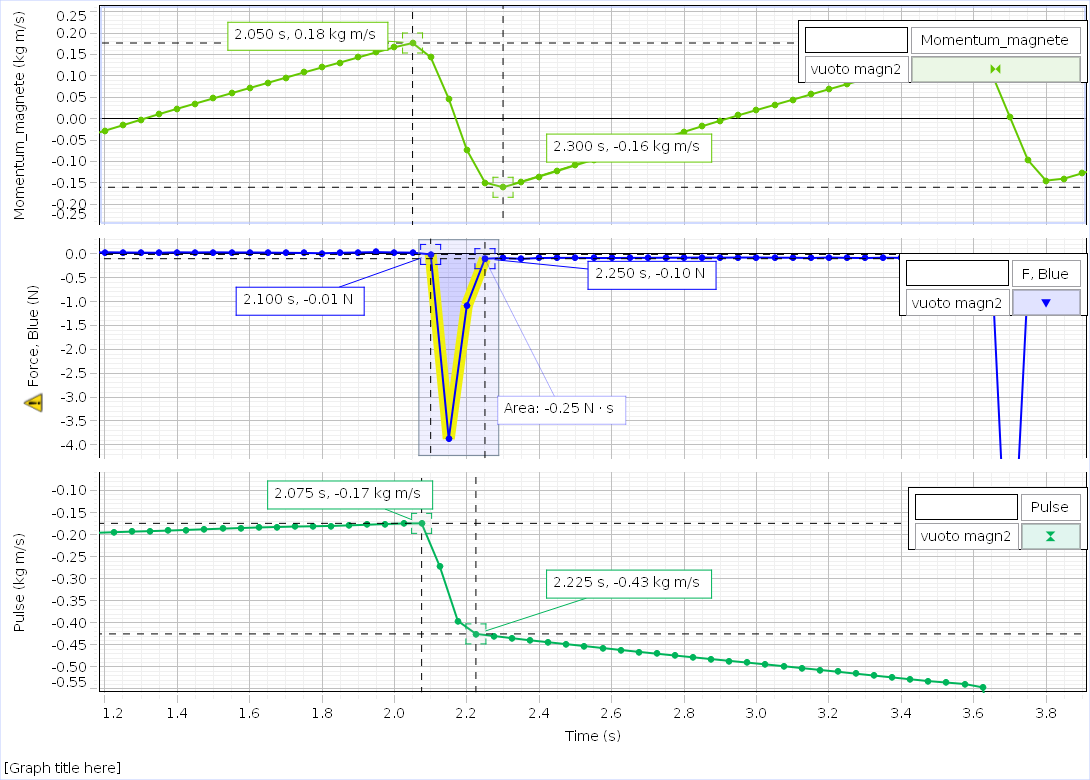
\includegraphics[scale=1.0]{capstone_data/magn_2.png}
			\end{subfigure}%
		}
	}
\end{figure}

\begin{figure}[!htbp]
	\captionsetup{labelformat= empty}
	\captionsetup[sub]{font=huge}
	
	\makebox[1 \textwidth][c]{       %centering table
		\resizebox{1.60 \textwidth}{!}{
			\begin{subfigure}{2.0\textwidth}
				\caption{run3}
				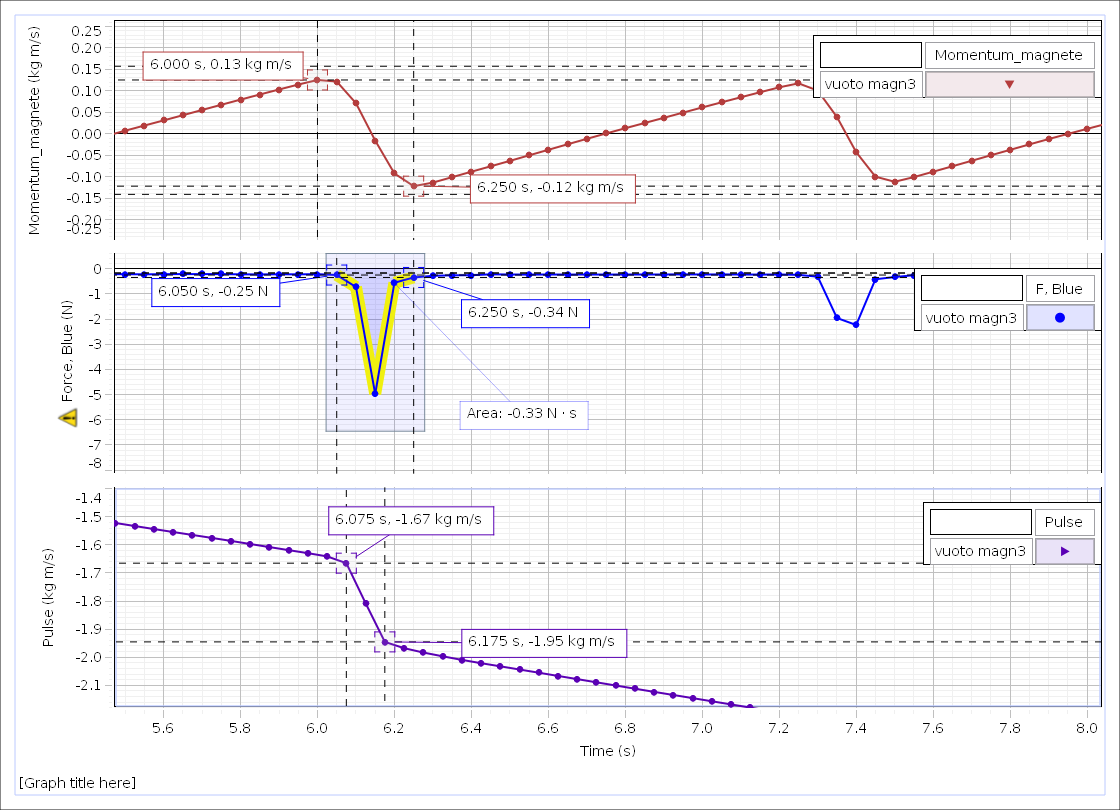
\includegraphics[scale=1.0]{capstone_data/magn_3.png}
			\end{subfigure}%
			
			\begin{subfigure}{2.0\textwidth}
				\caption{run 4}
				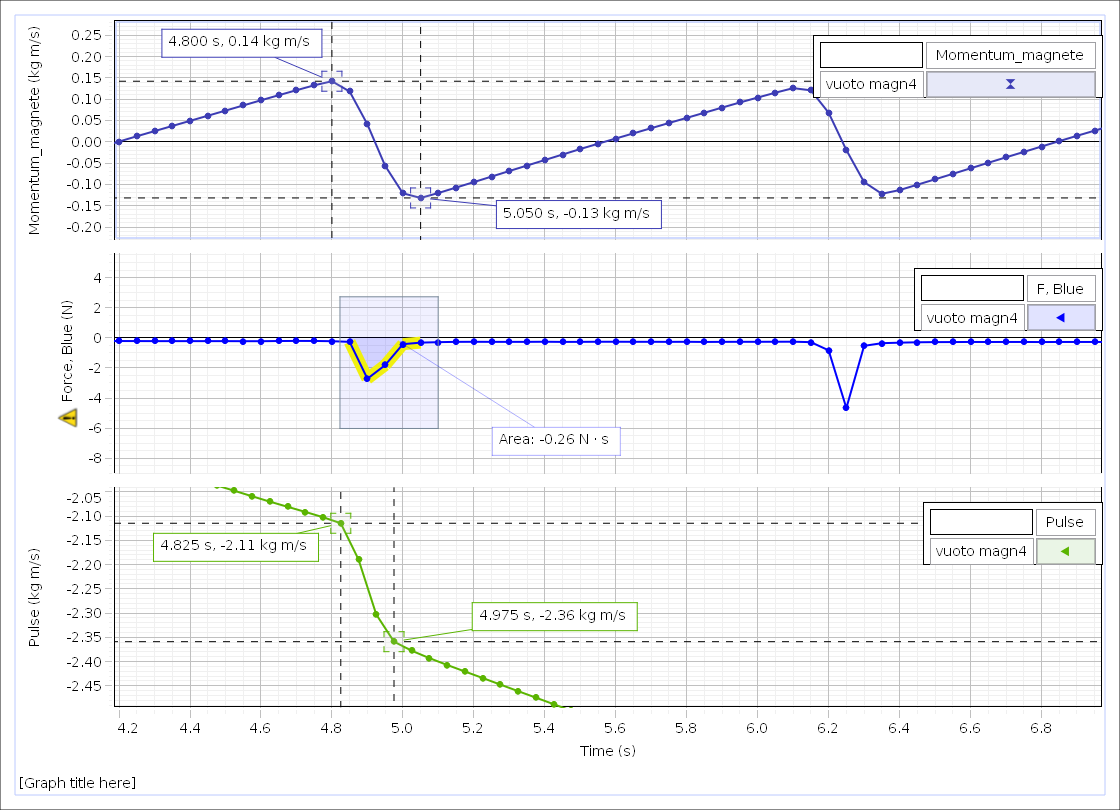
\includegraphics[scale=1.0]{capstone_data/magn_4.png}
			\end{subfigure}%
			
		}
	}
\end{figure}

\begin{figure}[!htbp]
	\captionsetup{labelformat= empty}
	\captionsetup[sub]{font=LARGE}
	
	\makebox[1 \textwidth][c]{       %centering table
		\resizebox{0.89\textwidth}{!}{
			\begin{subfigure}{2.0\textwidth}
				\caption{run 5}
				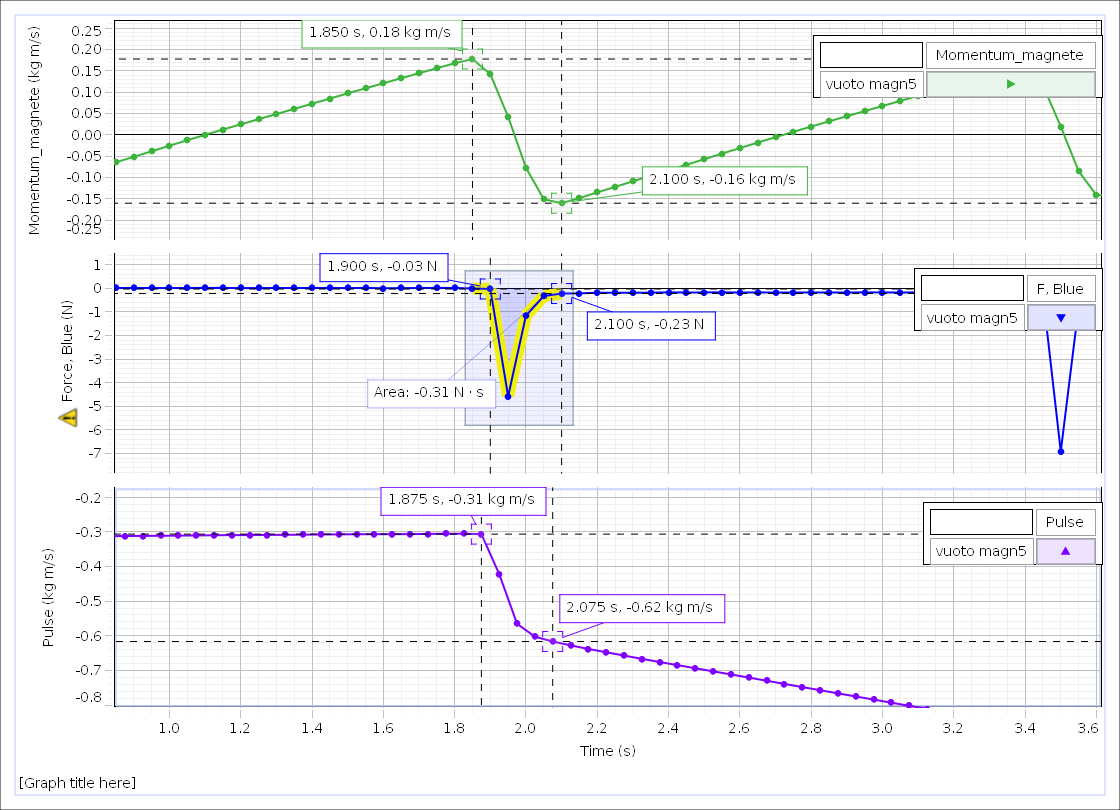
\includegraphics[scale=1.0]{capstone_data/magn_5.png}
			\end{subfigure}%
		}
	}
\end{figure}

\begin{figure}[!htbp]
		\captionsetup{labelformat= empty}
		\caption{verifica teorema dell'impulso con il magnete}
	\makebox[1 \textwidth][c]{       %centering table
		\begin{tabular}{||ccc||}
			\hline
			\hline
			run & \(\Delta p\) (Kg m/s) & I (N s)\\
			\hline
			1: & -0.15-0.15 = -0.30 & -0.21\\
			2: & -0.16-0.18 = -0.34 & -0.25\\
			3: & -0.12-0.13 = -0.25 & -0.33\\
			4: & -0.13-0.14 = -0.27 & -0.26\\
			5: & -0.16-0.18 = -0.34 & -0.31\\
			\hline
			\hline
		\end{tabular}
		
	} %close centering
\end{figure}

%----------------------???--------------------
\[t = \frac{\left | \bar{I} - \bar{\Delta p} \right |}{\sqrt{\sigma_{I}^{2}+\sigma_{\Delta p}^{2}}}= \frac{0.028}{\sqrt{0.018^{2}+0.022^{2}}}= 0.99\]\\
\noindent \(\rightarrow\) la probabilità che la differenza sia dovuta solo ad errori casuali è del 32.2\(\%\).\\\\

\subsubsection*{verifica della conservazione dell'energia}
\begin{figure}[!htbp]
	\captionsetup{labelformat= empty}
	\captionsetup[sub]{font=huge}
	
	\caption{Grafici di \(v^{2}_{(t)}\) per il run 1}
	\makebox[1 \textwidth][c]{       %centering table
		\resizebox{1.70 \textwidth}{!}{
			\begin{subfigure}{1.8\textwidth}
				\caption{molla}
				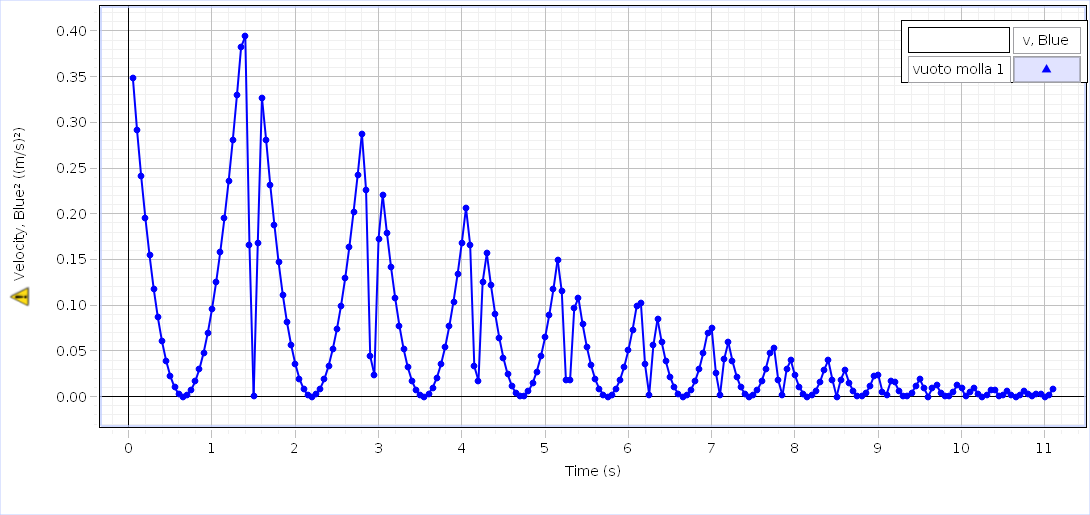
\includegraphics[scale=0.9]{capstone_data/v_quadro_molla.png}
			\end{subfigure}%
			
			\begin{subfigure}{1.8\textwidth}
				\caption{magnete}
				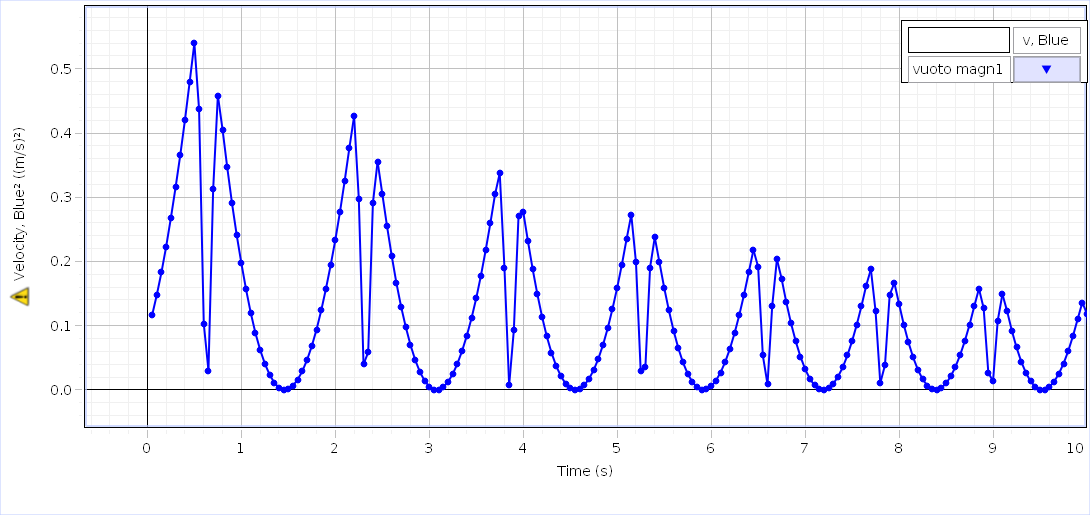
\includegraphics[scale=0.9]{capstone_data/v_quadro_magn.png}
			\end{subfigure}%
		}
	}
\end{figure}



\begin{figure}[!htbp]
	\captionsetup{labelformat= empty}
	\captionsetup[sub]{font=LARGE}
	
	\caption{Grafici dell'Energia Cinetica con la molla}
	\makebox[1 \textwidth][c]{       %centering table
		\resizebox{1.70 \textwidth}{!}{
			\begin{subfigure}{2.0\textwidth}
				\caption{run 1}
				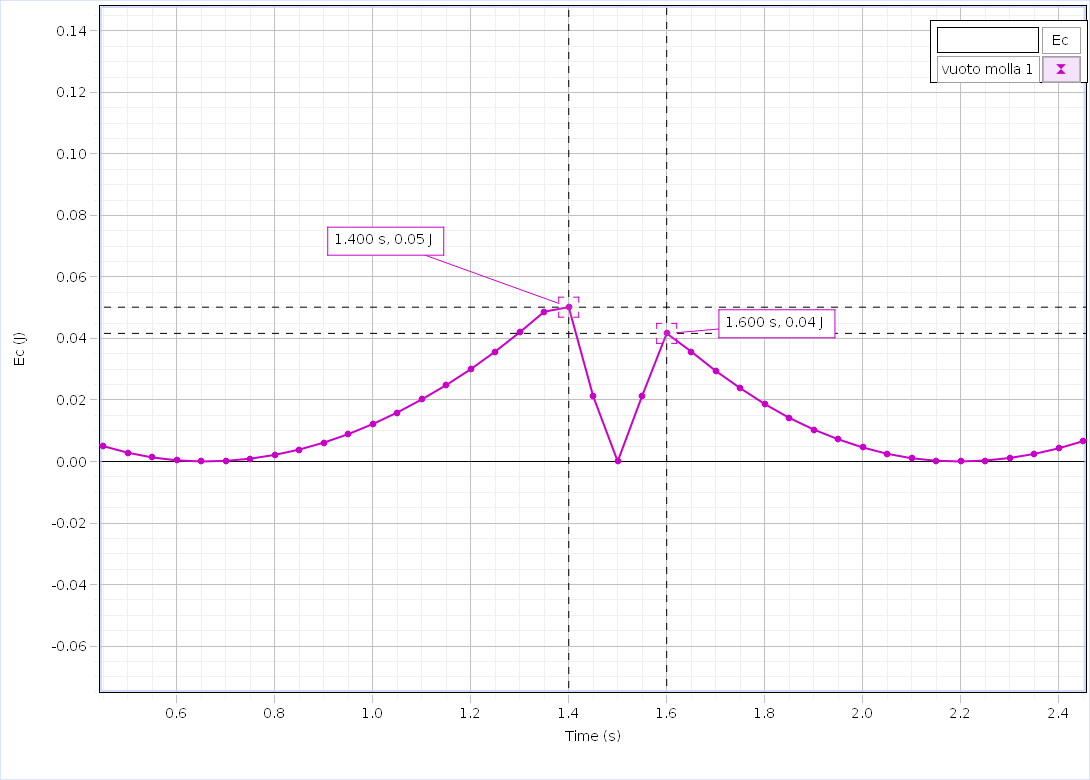
\includegraphics[scale=1.0]{capstone_data/Ec_molla_1.png}
			\end{subfigure}%
			
			\begin{subfigure}{2.0\textwidth}
				\caption{run 2}
				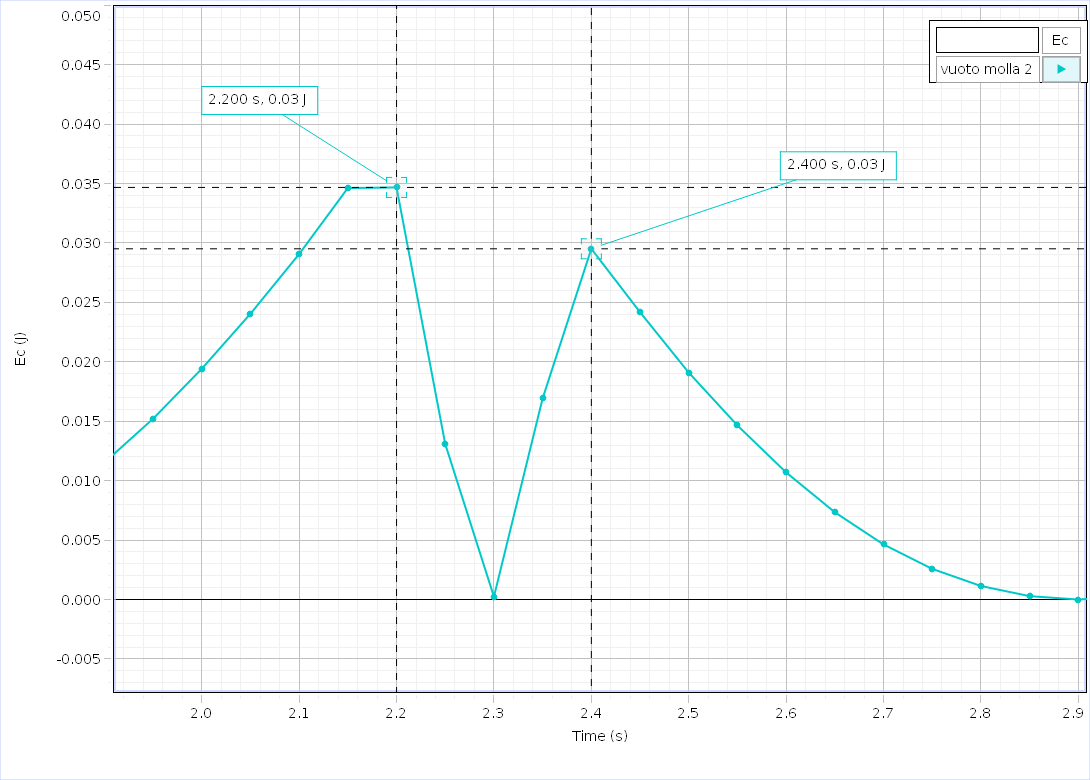
\includegraphics[scale=1.0]{capstone_data/Ec_molla_2.png}
			\end{subfigure}%
		}
	}
\end{figure}

\begin{figure}[!htbp]
	\captionsetup{labelformat= empty}
	\captionsetup[sub]{font=huge}
	
	\makebox[1 \textwidth][c]{       %centering table
		\resizebox{1.60 \textwidth}{!}{
			\begin{subfigure}{2.2\textwidth}
				\caption{run3}
				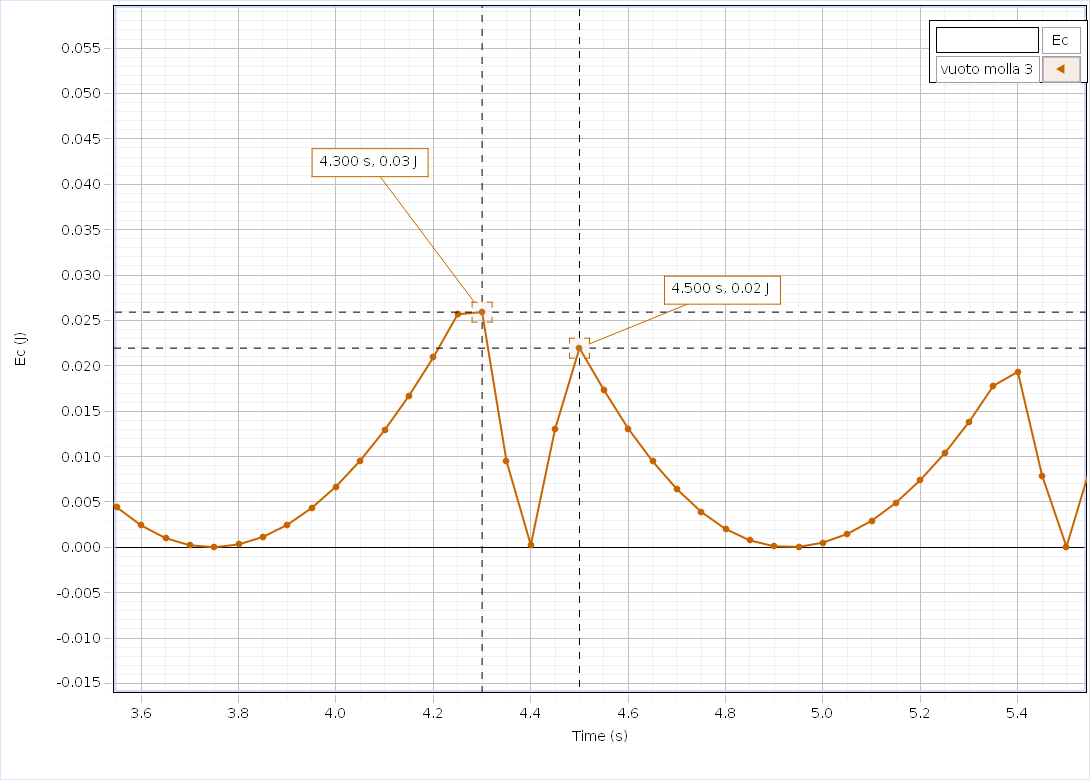
\includegraphics[scale=1.15]{capstone_data/Ec_molla_3.png}
			\end{subfigure}%
			
			\begin{subfigure}{2.2\textwidth}
				\caption{run 4}
				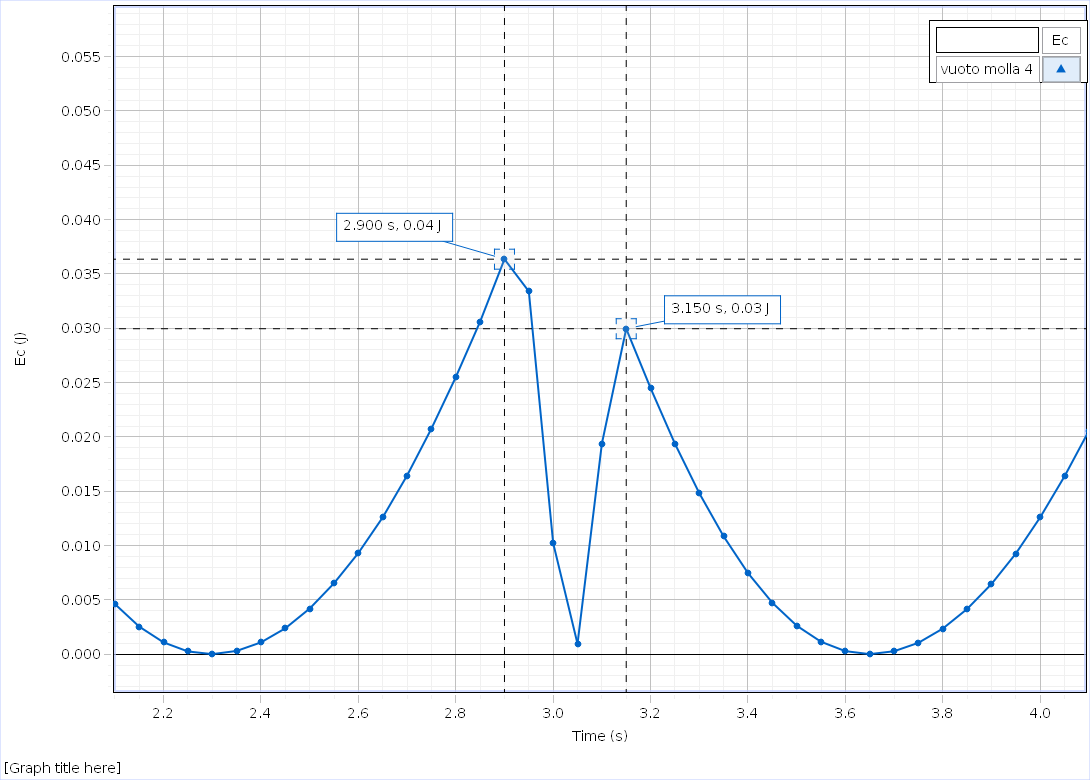
\includegraphics[scale=1.15]{capstone_data/Ec_molla_4.png}
			\end{subfigure}%
		
			\begin{subfigure}{2.2\textwidth}
				\caption{run 5}
				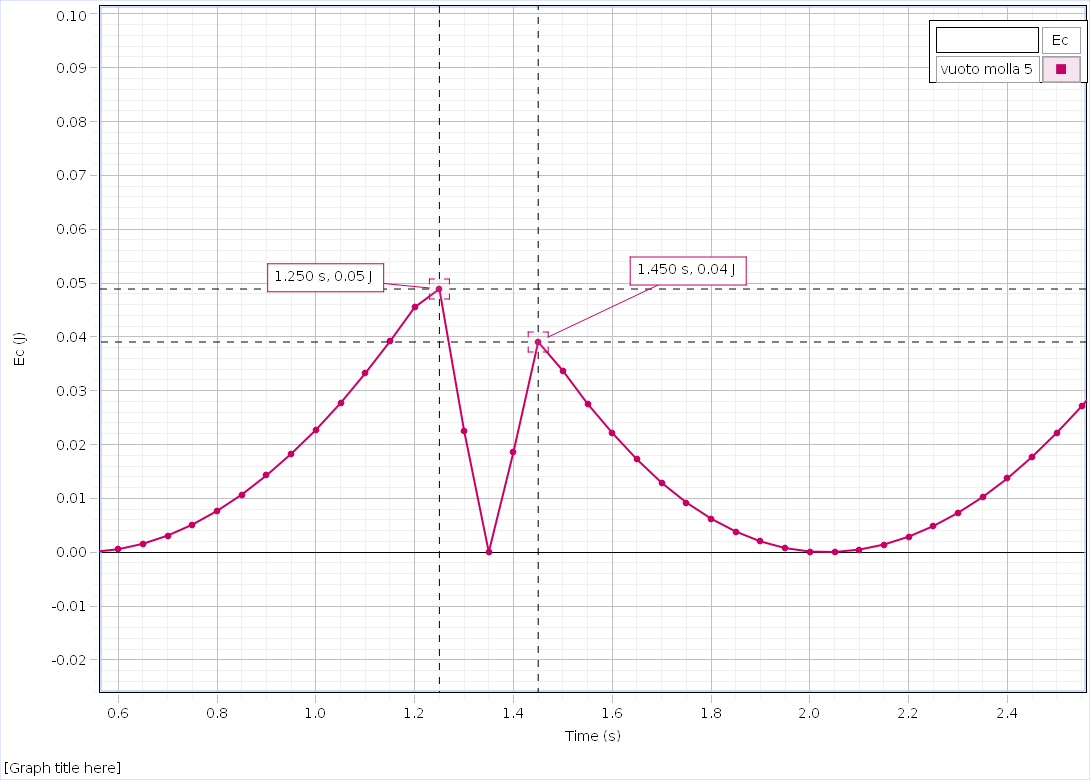
\includegraphics[scale=1.15]{capstone_data/Ec_molla_5.png}
			\end{subfigure}%
			
		}
	}
\end{figure}

\begin{figure}[!htbp]
	\captionsetup{labelformat= empty}
	\caption{verifica conservazione dell'energia con la molla}
	\makebox[1 \textwidth][c]{       %centering table
		\begin{tabular}{||cc||}
			\hline
			\hline
			run & \(\Delta Ec\) (J)\\
			\hline
			1: & 0.042-0.050 = -0.008 \\
			2: & 0.030-0.035 = -0.005\\
			3: & 0.022-0.026 = -0.004\\
			4: & 0.030- 0.036 = -0.006\\
			5: & 0.039-0.049 = -0.01\\
			\hline
			\hline
		\end{tabular}
		
	} %close centering
\end{figure}
.\\
\[t = \frac{ \left |\bar{\Delta_{Ec} - 0} \right |}{\sigma_{\Delta Ec}} = \frac{0.0066}{0.001} = 6.6\]
\noindent \(\rightarrow\) la probabilità che la differenza sia dovuta solo ad errori casuali è inferiore al 0.3\(\%\), risultato non accettabile.\\\\

\begin{figure}[!htbp]
	\captionsetup{labelformat= empty}
	\captionsetup[sub]{font=LARGE}
	
	\caption{Grafici dell'Energia Cinetica con il magnete}
	\makebox[1 \textwidth][c]{       %centering table
		\resizebox{1.70 \textwidth}{!}{
			\begin{subfigure}{2.0\textwidth}
				\caption{run 1}
				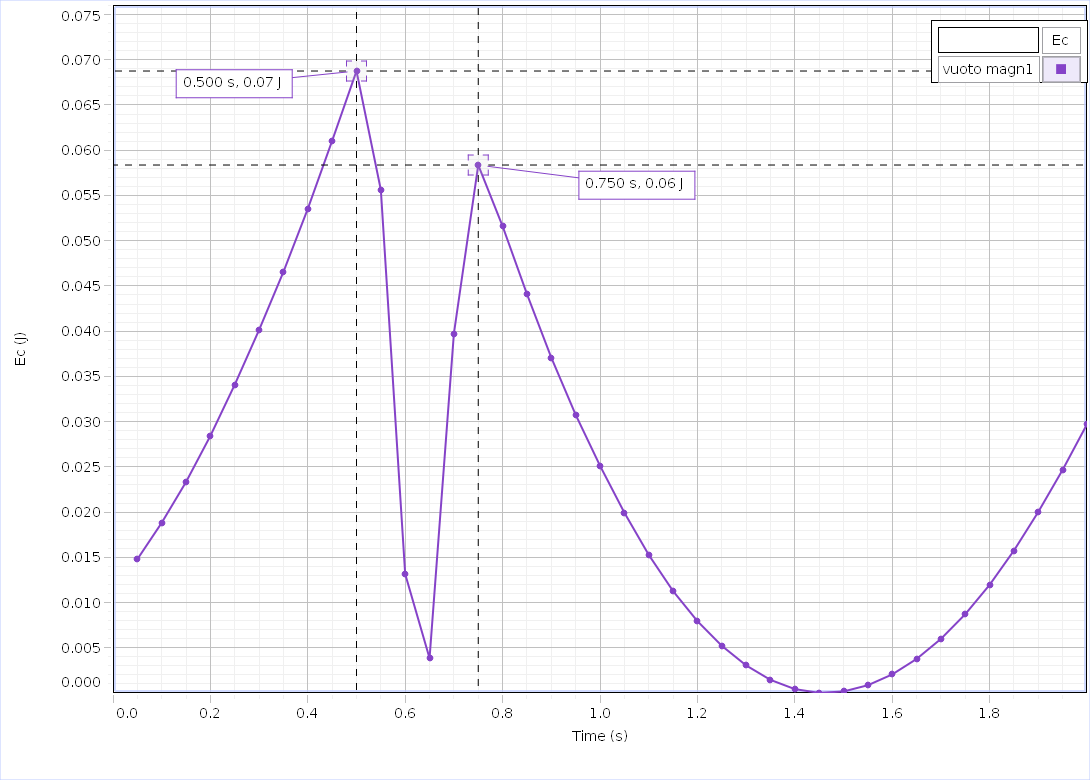
\includegraphics[scale=1.0]{capstone_data/Ec_magn_1.png}
			\end{subfigure}%
			
			\begin{subfigure}{2.0\textwidth}
				\caption{run 2}
				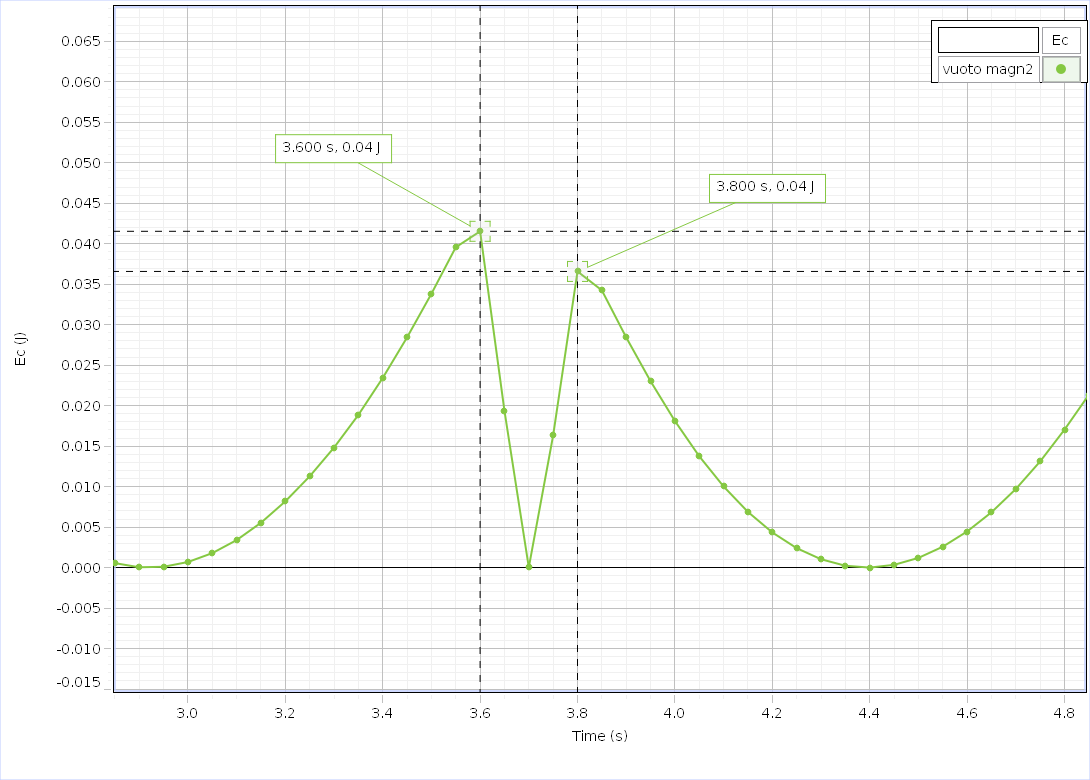
\includegraphics[scale=1.0]{capstone_data/Ec_magn_2.png}
			\end{subfigure}%
		}
	}
\end{figure}

\begin{figure}[!htbp]
	\captionsetup{labelformat= empty}
	\captionsetup[sub]{font=huge}
	
	\makebox[1 \textwidth][c]{       %centering table
		\resizebox{1.60 \textwidth}{!}{
			\begin{subfigure}{2.2\textwidth}
				\caption{run3}
				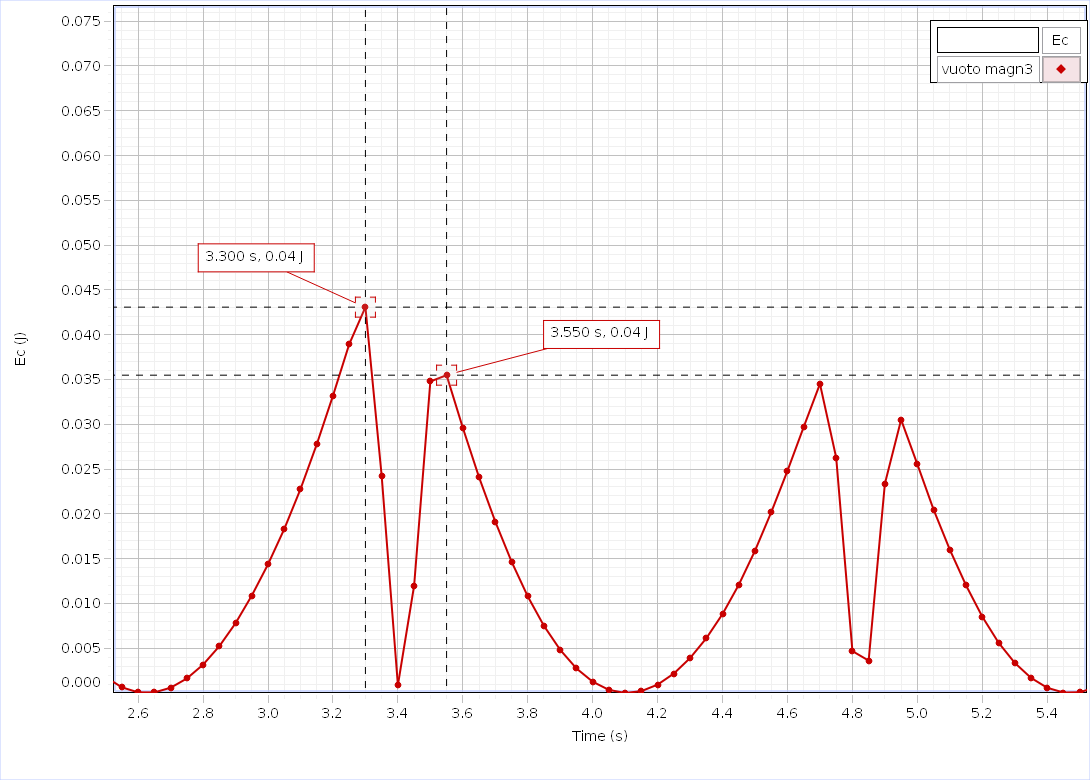
\includegraphics[scale=1.15]{capstone_data/Ec_magn_3.png}
			\end{subfigure}%
			
			\begin{subfigure}{2.2\textwidth}
				\caption{run 4}
				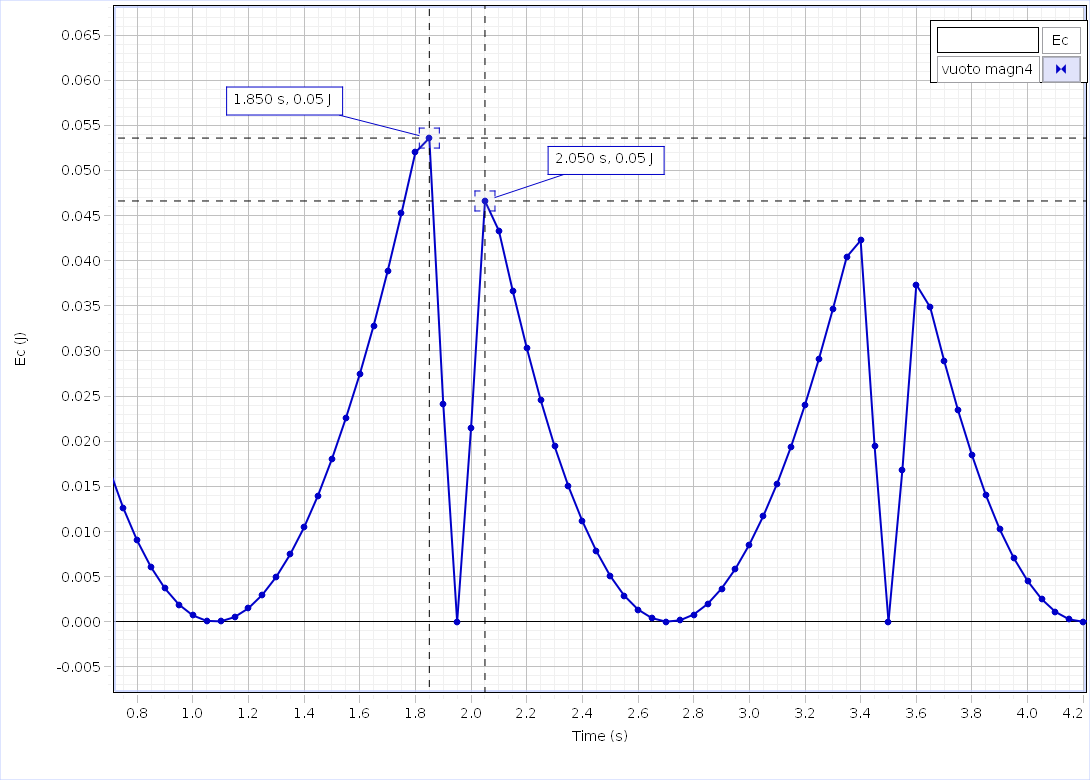
\includegraphics[scale=1.15]{capstone_data/Ec_magn_4.png}
			\end{subfigure}%
			
			\begin{subfigure}{2.2\textwidth}
				\caption{run 5}
				\includegraphics[scale=1.15]{capstone_data/Ec_magn_5.png}
			\end{subfigure}%
			
		}
	}
\end{figure}

\begin{figure}[!htbp]
	\captionsetup{labelformat= empty}
	\caption{verifica della conservazione dell'energia con il magnete}
	\makebox[1 \textwidth][c]{       %centering table
		\begin{tabular}{||cc||}
			\hline
			\hline
			run & \(\Delta Ec\) (J)\\
			\hline
			1: & 0.058-0.069 = -0.011\\
			2: & 0.037-0.042 = -0.005\\
			3: & 0.036- 0.043 = -0.007 \\
			4: & 0.047-0.054 = -0.007\\
			5: & 0.045-0.055 = -0.010\\
			\hline
			\hline
		\end{tabular}
		
	} %close centering
\end{figure}
.\\\\\\\\\\\\\\\\\\\\\\\\\\\\\\\\\\\\
\[t = \frac{ \left |\bar{\Delta_{Ec} - 0} \right |}{\sigma_{\Delta Ec}} = \frac{0.008}{0.001} = 8\]
\noindent \(\rightarrow\) la probabilità che la differenza sia dovuta solo ad errori casuali è inferiore al 0.3\(\%\), risultato non accettabile.\\\\

\subsection*{urti tra due carrelli}

\begin{figure}[!ht]
	\captionsetup{labelformat=empty}
	\caption{Grafico \(v_{(t)}\) run 1 urto elastico}
	\makebox[1 \textwidth][c]{       %centering table
		\resizebox{0.90 \textwidth}{!}{   %resize table
			\includegraphics{capstone_data/elastico_vel.png}
		} %close resize
	} %close centering
	
\end{figure}
\[v_{f R} = v_{i B} \frac{2 m_{B}}{m_{R}+m_{B}}\]
\begin{minipage}[c]{0.5\textwidth}
	\captionsetup{labelformat=empty}
	\captionof{table}{carrello blu \(v_{f} = 0\)}
	\centering
	\begin{tabular}{||cc||}
		\hline
		\hline
		run &  \(v_{i}\) (m/s)\\
		\hline
		1: & 0.531  \\ 
		2: & 0.474\\
		3: & 0.380\\
		4: & 0.558\\
		5: & 0.642\\
		\hline
		\hline
	\end{tabular}
	
\end{minipage}
\begin{minipage}[c]{0.5\textwidth}
	\captionsetup{labelformat=empty}
	\captionof{table}{carrello rosso \(v_{i} = 0\)}
	\centering
	\begin{tabular}{||ccc||}
		\hline
		\hline
		run &  \(v_{fosservata}\) (m/s) & \(v_{fattesa}\) (m/s)\\
		\hline
		1: & 0.516 & 0.528 \\
		2: & 0.469& 0.472\\
		3: & 0.368& 0.378\\
		4: & 0.544& 0.555\\
		5: & 0.618& 0.639\\
		\hline
		\hline
	\end{tabular}
\end{minipage}

\[v_{f R} = v_{i B} \frac{2 (0.270 Kg)}{0.543 Kg}\]

\[t = \frac{ \left |\bar{v_{oss}}  - \bar{v_{att}} \right |}{\sqrt{\sigma_{vosservata}^{2}+ \sigma_{vattesa}^{2}}} = 0.19\]
\noindent \(\rightarrow\) la probabilità che la differenza sia dovuta solo ad errori casuali è del 85\(\%\).\\\\

\begin{figure}[!ht]
	\captionsetup{labelformat=empty}
	\caption{Grafico \(v_{(t)}\) run 1 urto elastico (con carrello blu caricato con 500g)}
	\makebox[1 \textwidth][c]{       %centering table
		\resizebox{0.90 \textwidth}{!}{   %resize table
			\includegraphics{capstone_data/elastico_500_blu_vel.png}
		} %close resize
	} %close centering
	
\end{figure}

\begin{minipage}[c]{0.5\textwidth}
	\captionsetup{labelformat=empty}
	\captionof{table}{carrello blu \(v_{f} = 0\)}
	\centering
	\begin{tabular}{||cc||}
		\hline
		\hline
		run &  \(v_{i}\) (m/s)\\
		\hline
		1: & 0.524   \\ 
		2: & 0.400\\
		3: & 0.376\\
		4: & 0.612\\
		5: & 0.829\\
		\hline
		\hline
	\end{tabular}
	
\end{minipage}
\begin{minipage}[c]{0.5\textwidth}
	\captionsetup{labelformat=empty}
	\captionof{table}{carrello rosso \(v_{i} = 0\)}
	\centering
	\begin{tabular}{||ccc||}
		\hline
		\hline
		run &  \(v_{fosservata}\) (m/s) & \(v_{fattesa}\) (m/s)\\
		\hline
		1: & 0.752 & 0.775 \\
		2: &0.576& 0.592\\
		3: &0.543& 0.556\\
		4: & 0.881& 0.906\\
		5: &0.808& 0.828\\
		\hline
		\hline
	\end{tabular}
\end{minipage}

\[v_{f R} = v_{i B} \frac{2 (0.777 Kg)}{1.050 Kg}\]

\[t = \frac{ \left |\bar{v_{oss}}  - \bar{v_{att}} \right |}{\sqrt{\sigma_{vosservata}^{2}+ \sigma_{vattesa}^{2}}} = 0.2 \]
\noindent \(\rightarrow\) la probabilità che la differenza sia dovuta solo ad errori casuali è del 84\(\%\).\\\\\\\\\\\\\\\\\\
\begin{figure}[!ht]
	\captionsetup{labelformat=empty}
	\caption{Grafico \(v_{(t)}\) run 1 urto elastico (con carrello rosso caricato con 500g)}
	\makebox[1 \textwidth][c]{       %centering table
		\resizebox{0.90 \textwidth}{!}{   %resize table
			\includegraphics{capstone_data/elastico_500_rosso_vel.png}
		} %close resize
	} %close centering
	
\end{figure}

\begin{minipage}[c]{0.5\textwidth}
	\captionsetup{labelformat=empty}
	\captionof{table}{carrello blu \(v_{f} = 0\)}
	\centering
	\begin{tabular}{||cc||}
		\hline
		\hline
		run &  \(v_{i}\) (m/s)\\
		\hline
		1: &0.635  \\ 
		2: &0.640 \\
		3: &0.405 \\
		4: &0.547\\
		5: &0.528 \\
		\hline
		\hline
	\end{tabular}
	
\end{minipage}
\begin{minipage}[c]{0.5\textwidth}
	\captionsetup{labelformat=empty}
	\captionof{table}{carrello rosso \(v_{i} = 0\)}
	\centering
	\begin{tabular}{||ccc||}
		\hline
		\hline
		run &  \(v_{fosservata}\) (m/s) & \(v_{fattesa}\) (m/s)\\
		\hline
		1: &0.315  & 0.327\\
		2: &0.320 &0.330\\
		3: &0.201&0.209\\
		4: &0.277 &0.282\\
		5: & 0.264&0.272\\
		\hline
		\hline
	\end{tabular}
\end{minipage}

\[v_{f R} = v_{i B} \frac{2 (0.270 Kg)}{1.050 Kg}\]

\[t = \frac{ \left |\bar{v_{oss}}  - \bar{v_{att}} \right |}{\sqrt{\sigma_{vosservata}^{2}+ \sigma_{vattesa}^{2}}} = 0.28 \]
\noindent \(\rightarrow\) la probabilità che la differenza sia dovuta solo ad errori casuali è del 78\(\%\).\\\\\\\\\\\\\\\\\\\\\\\\


\begin{figure}[!htbp]
	\captionsetup{labelformat=empty}
	\caption{urto anaelastico (carrelli vuoti, \(v_{iR} = 0\))}
	\makebox[1 \textwidth][c]{       %centering table
		\resizebox{1.70 \textwidth}{!}{
			\begin{subfigure}{0.9\textwidth}
				\caption{quantità di moto}
				\includegraphics[scale=0.45]{capstone_data/anaelastico_momento.png}
			\end{subfigure}%
			
			\begin{subfigure}{0.9\textwidth}
				\caption{energia cinetica}
				\includegraphics[scale=0.45]{capstone_data/anaelastico_Ec.png}
			\end{subfigure}%
		}
	}
\end{figure}



\begin{figure}[!htbp]
	\captionsetup{labelformat=empty}
	\caption{Tabella variazione della quantità di moto con carrelli vuoti}
	\makebox[1 \textwidth][c]{ 
		\begin{tabular}{||ccc|c||}
			\hline
			\hline
			run &  \(\Delta p\)  carrello blu (Kg m/s) & \(\Delta p\)  carrello rosso (Kg m/s)& \(\Delta p\)  totale (Kg m/s)\\
			\hline
			1: &0.055-0.110 = -0.055 & 0.054-0 =  0.054 & -0.001\\ 
			2: &0.060-0.121 = -0.061& 0.061-0 =   0.061& 0\\
			3: &0.060-0.123 = -0.063 & 0.060-0 = 0.060 & -0.003\\
			4: &0.052-0.108 = -0.056 & 0.053-0 = 0.053 & -0.003\\
			5: &0.072-0.148 = -0.076& 0.073-0 = 0.073& -0.003\\
			\hline
			\hline
		\end{tabular}
	} %close centering
\end{figure}

\[t = \frac{\left | \bar{\Delta p} - 0\right |}{\sigma_{\Delta p}} = 3.3\]
\noindent \(\rightarrow\) la probabilità che la discrepanza con \(\Delta p = 0\) sia dovuto solo ad errori casuali è del 0.1 \(\%\), risultato non accettabile.
\begin{figure}[!htbp]
	\captionsetup{labelformat=empty}
	\caption{Tabella variazione della energia cinetica con carrelli vuoti}
	\makebox[1 \textwidth][c]{ 
		\begin{tabular}{||ccc|c||}
			\hline
			\hline
			run &  \(\Delta Ec\)  carrello blu (J) & \(\Delta Ec\)  carrello rosso (J) & \(\Delta Ec\)  totale (J)\\
			\hline
			1: & 0.005-0.022 = -0.017&0.0054-0 = 0.0054 & -0.012 \\ 
			2: &0.006-0.027 = -0.021 & 0.0067-0 = 0.0067& -0.014\\
			3: &0.007-0.028 = -0.021&0.007-0 = 0.007 & -0.014\\
			4: &0.0049-0.0214 = -0.017 & 0.005-0 = 0.005& -0.012\\
			5: &0.010-0.040 = -0.030 & 0.010-0 = 0.010 & -0.02 \\
			\hline
			\hline
		\end{tabular}
	} %close centering
\end{figure}

\begin{figure}[!htbp]
	\captionsetup{labelformat=empty}
	\caption{urto anaelastico (carrello blu caricato con 500g, \(v_{iR} = 0\))}
	\makebox[1 \textwidth][c]{       %centering table
		\resizebox{1.70 \textwidth}{!}{
			\begin{subfigure}{0.9\textwidth}
				\caption{quantità di moto}
				\includegraphics[scale=0.45]{capstone_data/anaelastico_500_blu_momento.png}
			\end{subfigure}%
			
			\begin{subfigure}{0.9\textwidth}
				\caption{energia cinetica}
				\includegraphics[scale=0.45]{capstone_data/anaelastico_500_blu_Ec.png}
			\end{subfigure}%
		}
	}
\end{figure}



\begin{figure}[!htbp]
	\captionsetup{labelformat=empty}
	\caption{Tabella variazione della quantità di moto con carrello blu caricato di 500g}
	\makebox[1 \textwidth][c]{ 
		\begin{tabular}{||ccc|c||}
			\hline
			\hline
			run &  \(\Delta p\)  carrello blu (Kg m/s) & \(\Delta p\)  carrello rosso (Kg m/s)& \(\Delta p\)  totale (Kg m/s)\\
			\hline
			1: &0.200-0.272 = -0.072& 0.071-0 = 0.071& -0.001\\
			2: &0.328-0.456 = -0.128 &0.114-0 = 0.114& -0.014\\
			3: &0.213-0.295 = -0.082& 0.076-0 = 0.076&-0.006\\
			4: &0.227-0.311 = -0.084 & 0.0813-0 = 0.081& -0.003\\
			5: &0.233-0.317 = -0.084& 0.082-0 = 0.082 &-0.002\\
			\hline
			\hline
		\end{tabular}
	} %close centering
\end{figure}

\[t = \frac{\left | \bar{\Delta p} - 0\right |}{\sigma_{\Delta p}} = 2.2\]
\noindent \(\rightarrow\) la probabilità che la discrepanza con \(\Delta p = 0\) sia dovuto solo ad errori casuali è del 3\(\%\), risultato accettabile.


\begin{figure}[!htbp]
	\captionsetup{labelformat=empty}
	\caption{Tabella variazione della energia cinetica con carrello blu caricato di 500g}
	\makebox[1 \textwidth][c]{ 
		\begin{tabular}{||ccc|c||}
			\hline
			\hline
			run &  \(\Delta Ec\)  carrello blu (J) & \(\Delta Ec\)  carrello rosso (J) & \(\Delta Ec\)  totale (J)\\
			\hline
			1: & 0.025-0.048 = -0.023 &0.009-0 = 0.009 & -0.014\\
			2: & 0.069-0.134 = -0.065& 0.024-0 = 0.024 & 0.041\\
			3: &0.029-0.056 = -0.027& 0.011-0 = 0.011 & -0.016\\
			4: & 0.033-0.062 = -0.029& 0.012-0 = 0.012& -0.017\\
			5:&0.035-0.065 = -0.030 & 0.012-0 = 0.012 & -0.018\\
			\hline
			\hline
		\end{tabular}
	} %close centering
\end{figure}

\begin{figure}[!htbp]
	\captionsetup{labelformat=empty}
	\caption{urto anaelastico (carrello rosso caricato con 500g, \(v_{iR} = 0\))}
	\makebox[1 \textwidth][c]{       %centering table
		\resizebox{1.70 \textwidth}{!}{
			\begin{subfigure}{0.9\textwidth}
				\caption{quantità di moto}
				\includegraphics[scale=0.45]{capstone_data/anaelastico_500_rosso_momento.png}
			\end{subfigure}%
			
			\begin{subfigure}{0.9\textwidth}
				\caption{energia cinetica}
				\includegraphics[scale=0.45]{capstone_data/anaelastico_500_rosso_Ec.png}
			\end{subfigure}%
		}
	}
\end{figure}



\begin{figure}[!htbp]
	\captionsetup{labelformat=empty}
	\caption{Tabella variazione della quantità di moto con carrello rosso caricato con 500g}
	\makebox[1 \textwidth][c]{ 
		\begin{tabular}{||ccc|c||}
			\hline
			\hline
			run &  \(\Delta p\)  carrello blu (Kg m/s) & \(\Delta p\)  carrello rosso (Kg m/s)& \(\Delta p\)  totale (Kg m/s)\\
			\hline
			1: & 0.040-0.156 = -0.116&0.116-0= 0.116 & 0\\
			2: &0.044-0.169 = -0.125& 0.126-0 = 0.126 & 0.001\\
			3: &0.049-0.188 = -0.139& 0.140-0 = 0.140 & 0.001\\
			4: & 0.039-0.162 = -0.123& 0.122-0 = 0.122 &-0.001\\
			5: & 0.050+0.202 = -0.152& 0.151- 0 = 0.151 &-0.001\\
			\hline
			\hline
		\end{tabular}
	} %close centering
\end{figure}

\[t = \frac{\left | \bar{\Delta p} - 0\right |}{\sigma_{\Delta p}} = 0\]
\noindent \(\rightarrow\) la probabilità che la discrepanza con \(\Delta p = 0\) nei diversi run sia dovuto solo ad errori casuali è del 100\(\%\).

\begin{figure}[!htbp]
	\captionsetup{labelformat=empty}
	\caption{Tabella variazione della energia cinetica con carrello rosso caricato con 500g}
	\makebox[1 \textwidth][c]{ 
		\begin{tabular}{||ccc|c||}
			\hline
			\hline
			run &  \(\Delta Ec\)  carrello blu (J) & \(\Delta Ec\)  carrello rosso (J) & \(\Delta Ec\)  totale (J)\\
			\hline
			1:& 0.003-0.045 = -0.042& 0.009- 0 = 0.009 & -0.033\\
			2: &0.004-0.053 = -0.049 & 0.010-0 = 0.010 &-0.039\\
			3: &0.004-0.065 = -0.061 &0.013-0 = 0.013 & -0.048\\
			4: & 0.003-0.048 = -0.045& 0.010-0 = 0.010 & -0.035\\
			5: & 0.005-0.075 = -0.070&0.015-0 = 0.015 & -0.055\\
			\hline
			\hline
		\end{tabular}
	} %close centering
\end{figure}

\subsection*{calcolo del coefficiente di attrito}

\begin{figure}[!ht]
	\captionsetup{labelformat=empty}
	\caption{Grafico \(F_{(x)}\) con un libro davanti al carrello sottoposto a tensione}
	\makebox[1 \textwidth][c]{       %centering table
		\resizebox{0.90 \textwidth}{!}{   %resize table
			\includegraphics{capstone_data/1libro.png}
		} %close resize
	} %close centering
	
\end{figure}
\noindent In questo esempio il valore della tensione applicata è 1.96 N (peso del pesetto da 200g). Quando il carrello è libero di muoversi la tensione tende a spostare il carrello in avanti, contrastando la forza di attrito del libro posto di fronte al carrello: la risultante ora non è più T=1.96N ma T-\(F_{a}\)=1.70N \(\Rightarrow\) \(F_{a} = 0.26N\) è la forza necessaria a spostare il carrello trattenuto dal libro.\\
\[\mu = \frac{F_{a}}{m_{libro}g} = 0.0055\]
.\\\\\\\\\\\\\\\\\\\\\\\\\\
\makebox[\textwidth]{
	{	
		\normalsize
abbiamo calcolato \(\mu\) per tutti i run eseguiti:
	}
}
\begin{figure}[!htbp]
	\captionsetup{labelformat=empty}
	\caption{1 Libro, \(m_{libro} = 0.482 Kg\)}
	\makebox[1 \textwidth][c]{ 
		\begin{tabular}{ccc}
			\hline
			\hline
			run & \(F_{a}\) (N)& \(\mu\)\\
			\hline
			1: & 0.26 & 0.055\\ 
			2: & 0.27 & 0.057\\
			3: &0.29 & 0.06\\
			4: &0.22 & 0.005\\
			5: & 0.13 & 0.027\\
			\hline
			\hline
		\end{tabular}
	} %close centering
	\caption{\(\bar{\mu} = 0.041 \pm 0.011\)}
\end{figure}

\begin{figure}[!ht]
	\captionsetup{labelformat=empty}
	\caption{Grafico \(F_{(x)}\) con due libri davanti al carrello sottoposto a tensione}
	\makebox[1 \textwidth][c]{       %centering table
		\resizebox{0.90 \textwidth}{!}{   %resize table
			\includegraphics{capstone_data/2libri.png}
		} %close resize
	} %close centering
	
\end{figure}
\noindent La formula per \(\mu\) è la stessa riportata sopra, \(m_{libri}\) è diverso
\begin{figure}[!htbp]
	\captionsetup{labelformat=empty}
	\caption{2 Libri, \(m_{libri tot} = 0.798 Kg\)}
	\makebox[1 \textwidth][c]{ 
		\begin{tabular}{ccc}
			\hline
			\hline
			run & \(F_{a}\) (N)& \(\mu\)\\
			\hline
			1: & 0.19 & 0.024\\ 
			2: & 0.19 & 0.024\\
			3: &0.04 & 0.005\\
			4: &0.10 & 0.013\\
			5: & 0.25 & 0.032\\
			\hline
			\hline
		\end{tabular}
	} %close centering
	\caption{\(\bar{\mu} = 0.0196 \pm 0.0047\)}
\end{figure}


\begin{figure}[!htbp]
	\captionsetup{labelformat=empty}
	\caption{Grafici \(v_{(t)}\) e \(x_{(t)}\) del carrello blu con molla, \(\theta = 12 ^{\circ}\)}
	\makebox[1 \textwidth][c]{       %centering table
		\resizebox{1.70 \textwidth}{!}{
			\begin{subfigure}{0.9\textwidth}
				\includegraphics[scale=0.45]{capstone_data/attrito1.png}
				\caption{discesa: coefficiente angolare = \(1.96 \pm 0.0014\)}
			\end{subfigure}%
			
			\begin{subfigure}{0.9\textwidth}
				\includegraphics[scale=0.45]{capstone_data/attrito2.png}
				\caption{salita: coefficiente angolare = \(2.05 \pm 0.0019\)}
			\end{subfigure}%
		}
	}
\end{figure}

\end{document}